%% CHI paper, ACM primary article template (acmart, sigconf).
%% For the anonymous review version, use:  \documentclass[sigconf,anonymous,review]{acmart}
\documentclass[sigconf]{acmart}

% %% ---- Conference information (CHI '27; location and dates still to be announced) ----
% \acmConference[CHI '27]{Proceedings of the CHI Conference on Human Factors in Computing Systems}{April 2027}{TBD}
% \acmYear{2027}
% \copyrightyear{2027}
% \acmDOI{XXXXXXX.XXXXXXX}
% \acmISBN{978-1-4503-XXXX-X/2027/04}
% \acmPrice{15.00}

%% ---- First page: no ACM reference format and no copyright/permission footnote ----
\settopmatter{printacmref=false}
\setcopyright{none}
\renewcommand\footnotetextcopyrightpermission[1]{}

%% ---- Packages ----
\usepackage{tikz}
\usetikzlibrary{arrows.meta, positioning, shapes.geometric, shapes.multipart, calc, fit, backgrounds, decorations.pathreplacing}
\usepackage{booktabs}
\usepackage{array}

%% ---- Diagram palette: colour marks what the user can perceive (blue), the hidden middle layer (orange),
%% the physical robot side (green) and failure reports (red). Line style and labels repeat the encoding,
%% so the figures stay readable in greyscale.
\definecolor{cInk}{HTML}{22303C}
\definecolor{cVis}{HTML}{E3EEF8}\definecolor{cVisD}{HTML}{2E6594}
\definecolor{cHid}{HTML}{FDEBD3}\definecolor{cHidD}{HTML}{B4601A}
\definecolor{cHw}{HTML}{E2F1E4}\definecolor{cHwD}{HTML}{2F7A47}
\definecolor{cBad}{HTML}{FBE4E1}\definecolor{cBadD}{HTML}{B03A2E}
\definecolor{cFb}{HTML}{5F4B9A}

\newcommand{\wmtag}[1]{{\fontsize{5.6}{6}\selectfont\bfseries\color{cBadD}#1}}
\newcommand{\dgtitle}[1]{{\bfseries #1}}

\tikzset{
  base/.style={rectangle, rounded corners=3pt, draw, line width=0.7pt, align=center,
               font=\scriptsize, text=cInk, inner sep=3pt, minimum height=1.05cm,
               text width=2.05cm},
  vis/.style={base, draw=cVisD, fill=cVis},
  hid/.style={base, draw=cHidD, fill=cHid},
  hw/.style={base, draw=cHwD, fill=cHw},
  store/.style={base, draw=cHwD, fill=white, dashed},
  backend/.style={base, draw=cHidD, fill=white, dashed, text width=1.55cm, minimum height=0.95cm},
  bad/.style={base, draw=cBadD, fill=cBad, dotted, line width=0.9pt},
  tag/.style={rectangle split, rectangle split parts=2, rectangle split draw splits=false},
  dec/.style={diamond, aspect=2.2, draw=cHidD, fill=white, line width=0.7pt, align=center,
              inner sep=0pt, text width=1.45cm, font=\scriptsize, text=cInk},
  snum/.style={circle, fill=cInk, text=white, font=\fontsize{5.5}{6}\selectfont\bfseries,
               inner sep=0pt, minimum size=3.5mm},
  main/.style={-{Stealth[length=2.1mm]}, line width=1pt, draw=cInk},
  aux/.style={-{Stealth[length=1.9mm]}, line width=0.75pt, densely dashed, draw=cInk!75},
  fb/.style={-{Stealth[length=1.9mm]}, line width=0.85pt, dashed, draw=cFb},
  lab/.style={font=\scriptsize, text=cInk},
}
\newcommand{\sn}[2]{\node[snum] at (#1.north west) {#2};}


\begin{document}

\title{Mind the Middle Layer: A Requirements-Driven Study of Wrong Mental Models in LLM-Agent-Controlled Robots}

\author{Md Akib Haider}
\authornote{These authors contributed equally to this work.}
\affiliation{%
  \department{Department of Computer Science and Engineering}
  \institution{Islamic University of Technology, Bangladesh}
}

\author{Nafis Fuad Shahid}
\authornotemark[1]
\affiliation{%
  \department{Department of Computer Science and Engineering}
  \institution{Islamic University of Technology, Bangladesh}
}

\author{Sakib Ahmed Shanto}
\authornotemark[1]
\affiliation{%
  \department{Department of Computer Science and Engineering}
  \institution{Islamic University of Technology, Bangladesh}
}

\author{Dr Hasan Mahmud}
\affiliation{%
  \department{Department of Computer Science and Engineering}
  \institution{Islamic University of Technology, Bangladesh}
}


\renewcommand{\shortauthors}{Haider et al.}

\begin{abstract}
People can now tell a robot what to do in plain language. Behind that request, a large language model (LLM) agent interprets it, writes microcontroller code for the specific robot, checks the code, and flashes it to the board. The user sees none of this. They speak, and the robot moves, or it does not. We argue that this hidden middle layer leads to wrong mental models. People place intelligence in the robot instead of the agent, blame the wrong part of the pipeline when something fails, and misjudge what the robot can safely do. Because the robot acts in the physical world, these mistakes matter more than they do for a chatbot.

This is a framework-and-plan paper, not an empirical study. We contribute a stakeholder and requirements analysis; a plug-and-play architecture in which a connection handshake registers the robot's capabilities and a validation stage runs before any flash; a taxonomy of seven wrong mental models drawn from the literature; a planned mixed-methods study of about one hundred participants to test that taxonomy; and mitigations tied to human--AI interaction guidelines, with an evaluation plan. We also built RoverLens, a simulator, and a scenario-based survey that tells participants where their understanding was wrong. The survey comes with an answer key, a catalogue of concrete cases for each wrong model, and a frame for reporting response statistics. No survey responses have been collected yet, and every participant example in the paper is hypothetical.
\end{abstract}

\begin{CCSXML}
<ccs2012>
<concept>
<concept_id>10003120.10003121</concept_id>
<concept_desc>Human-centered computing~Human computer interaction (HCI)</concept_desc>
<concept_significance>500</concept_significance>
</concept>
<concept>
<concept_id>10003120.10003121.10003122</concept_id>
<concept_desc>Human-centered computing~HCI design and evaluation methods</concept_desc>
<concept_significance>300</concept_significance>
</concept>
<concept>
<concept_id>10010520.10010553</concept_id>
<concept_desc>Computer systems organization~Embedded and cyber-physical systems</concept_desc>
<concept_significance>300</concept_significance>
</concept>
</ccs2012>
\end{CCSXML}

\ccsdesc[500]{Human-centered computing~Human computer interaction (HCI)}
\ccsdesc[300]{Human-centered computing~HCI design and evaluation methods}
\ccsdesc[300]{Computer systems organization~Embedded and cyber-physical systems}

\keywords{mental models; folk theories; human--robot interaction; large language models; LLM agents; natural-language robot programming; code generation; trust calibration; explainability; requirements engineering}

\maketitle

\section{Introduction}

Controlling a robot used to mean writing firmware. Now a growing number of systems let a person type or speak a command to an LLM agent, which works out the intent, writes control code for that particular robot, and runs it on the robot's microcontroller~\cite{liang2023code, singh2023progprompt, ahn2022saycan, vemprala2024chatgpt}. From the outside the exchange is short: the user talks, there is a pause, and the robot acts. Inside, several steps happen that nobody sees. The agent interprets the request, writes a program, validates it, compiles it, and flashes it to the hardware.

That invisibility is the design problem. Norman's framing is useful here: a system works when its \emph{system image} helps people cross the \emph{gulf of execution} (what can I do?) and the \emph{gulf of evaluation} (what just happened?)~\cite{hutchins1985direct, norman2013design}. A pipeline that hides its middle layer widens the second gulf. When the robot does something unexpected, the user has nothing to look at that would point to a cause. A mental model is a person's own account of how a system works. It is usually incomplete and often wrong, yet people act on it and set their expectations by it~\cite{norman1983some, kieras1984role, johnsonlaird1983mental, gero2020mental}. When the model is wrong, their actions and expectations drift away from what the system does, and they rarely notice. The quality of a person's model is linked to how well they work with an AI teammate~\cite{bansal2019beyond}, and conversational agents in particular show a documented gap between what people expect and what they get~\cite{luger2016like}.

We study one person operating one small robot, a wheeled or simple manipulator platform driven by an ESP32- or Arduino-class board, through an integrated agent. The main users have little or no robotics or programming background. Hobbyists and expert developers serve as comparison groups. The setting is short command episodes, and some of them fail. Because the robot is physical, a wrong model is more than an annoyance. Misjudging what the robot will do, or why it failed, can lead to unsafe actions or to throwing away hardware that works. That sets this problem apart from earlier mental-model work on recommender and conversational systems, where the stakes are mostly informational~\cite{eslami2015always, eslami2016first, gero2020mental}.

\subsection{Research Questions and Contribution}
We ask four questions. \textbf{RQ1}: What wrong mental models do non-expert users form of an agent~$\rightarrow$~code-generation~$\rightarrow$~hardware pipeline, and where do the errors cluster? \textbf{RQ2}: How do interface choices (voice or text, visible or hidden code, latency, failure messages) shape those models? \textbf{RQ3}: Can a wrong model be detected from behavior plus targeted probes, and does a detected flaw predict later errors? \textbf{RQ4}: Which mitigations repair the model and improve appropriate reliance without overwhelming the user?

This is a framework-and-plan paper: a theoretical and artifact contribution in the sense of Wobbrock and Kientz~\cite{wobbrock2016research}, not an empirical one. It reports no collected data. Its contributions are a requirements analysis grounded in the literature (\S\ref{sec:req}); a planned study and analysis (\S\ref{sec:data}--\S\ref{sec:analysis}); a plug-and-play architecture with a validate-before-flash stage, drawn as two diagrams (\S\ref{sec:design}); a taxonomy of seven wrong mental models (\S\ref{sec:taxonomy}); mitigations and an evaluation plan (\S\ref{sec:eval}); and an implemented simulator and understanding survey, with an answer key, a catalogue of cases for each category, and a frame for reporting response statistics (\S\ref{sec:survey}, \S\ref{sec:stats}, \S\ref{sec:cases}, Appendices~\ref{app:instrument}--\ref{app:key}). Because no study has been run yet, we introduce the failure modes in \S\ref{sec:req} as motivating observations and develop them fully as the taxonomy in \S\ref{sec:taxonomy}. The study in \S\ref{sec:data}--\S\ref{sec:analysis} is designed to test that taxonomy. \emph{All personas and numbers in \S\ref{sec:sample} are hypothetical worked examples, not findings, and the response tables in \S\ref{sec:stats} are empty because no responses exist.}

\section{Requirements, Stakeholders and Problem Space}\label{sec:req}

Requirements work starts by asking who is involved, what they do, and what they care about~\cite{preece2023interaction}. \emph{Primary users} are non-expert operators who give commands and try to make sense of what happens. \emph{Secondary users} are hobbyists and expert developers, who serve as comparison groups and may extend the system. \emph{Deployers} (educators, lab supervisors, product integrators) install the agent on a robot and answer for its behavior. \emph{Domain experts} in robotics and NLP inform the capability model. These groups want different things. A primary user wants predictability and an easy way to recover. A deployer also needs safety. An integrator has to manage the cost and latency of a remote model.

We keep a risk register of assumptions, each marked as backed by evidence, uncertain, or still to be tested. \textbf{A1}: users will credit the robot with intelligence instead of the hidden agent. \textbf{A2}: users cannot tell a hardware fault from a code-generation fault without help. \textbf{A3}: users will assume the system can do anything they can put into words. Earlier work found that people are often unaware of invisible computational layers and invent folk theories to explain what they can see~\cite{eslami2015always, eslami2016first}, which fits A1--A3. Even so, we treat them as hypotheses for \S\ref{sec:data} to test, not as facts about this system.

Each motivating observation becomes a requirement that names an actor, a condition, and a success criterion, and each is tied to the literature instead of to our own preferences. Functional requirements describe what the system does. Data requirements say what must be recorded. Quality requirements cover reliability, learnability, and safety. Organizational requirements cover deployment and governance. Table~\ref{tab:req} lists the core set. Several follow directly from established human--AI guidelines: make clear what the system can do and why it acted, and support efficient correction and dismissal~\cite{amershi2019guidelines}. They also follow from the idea that automation should support \emph{appropriate} reliance, since both too much and too little trust cause harm~\cite{lee2004trust}. The failure surface behind R5--R8 is developed as a taxonomy in \S\ref{sec:taxonomy}.

\begin{table*}[t]
  \caption{Core requirements, each traced to evidence or literature. IDs are stable and referenced from the design (\S5), taxonomy (\S6), and mitigations (\S7).}
  \label{tab:req}
  \small
  \begin{tabular}{@{}p{0.7cm}p{1.7cm}p{7.6cm}p{4.3cm}p{1.2cm}@{}}
    \toprule
    ID & Type & Requirement & Evidence / rationale & Priority \\
    \midrule
    R1 & Functional & On robot connect, the system shall auto-register the device's identity and a machine-readable capability manifest (sensors, actuators, board type) without user configuration. & Plug-and-play lowers the barrier for non-experts; grounds later refusal (A3). & Must \\
    R2 & Functional & The agent shall refuse, with an explanation, any command outside the registered capability manifest, rather than attempting a partial or fabricated action. & Ungrounded LLMs otherwise produce unsafe or nonsensical actions~\cite{ahn2022saycan}; ``make clear what the system can do''~\cite{amershi2019guidelines}. & Must \\
    R3 & Quality (safety) & No generated code shall reach the microcontroller before passing static, dry-run, and safety validation. & A physical effector makes unchecked code a safety hazard. & Must \\
    R4 & Data & The system shall retain per-episode provenance (utterance, generated code, validation result, flash status, execution feedback) to support diagnosis and study analysis. & Enables distinguishing user confusion from genuine system failure (\S8.2). & Must \\
    R5 & Quality & The interface shall report failures with a distinguishable, layer-specific cause (input, capability, code, deployment, execution). & Users cannot otherwise localize faults (A2); supports appropriate reliance~\cite{lee2004trust}. & Must \\
    R6 & Quality & The interface shall make the hidden pipeline legible on request (e.g.\ ``generating code,'' ``uploading,'' ``running''). & Revealing an invisible layer reshapes users' models~\cite{eslami2015always}; ``make clear why the system did what it did''~\cite{amershi2019guidelines}. & Should \\
    R7 & Quality & The system shall expose the active session/context state so a user can see when earlier commands are no longer available. & Context-window limits silently break follow-ups~\cite{liu2024lost}. & Should \\
    R8 & Organizational & When the underlying model or firmware changes, the deployer shall be able to surface a change notice to users. & Silent change violates expectations and triggers resistance~\cite{devito2017algorithms}; ``notify users about changes''~\cite{amershi2019guidelines}. & Could \\
    \bottomrule
  \end{tabular}
\end{table*}

\section{Experiemntal Setup}\label{sec:data}

We plan a mixed-methods study because no single method captures a mental model well. Models are inferred, not observed~\cite{gero2020mental, tabrez2020survey}. Think-aloud during use shows reasoning as it happens~\cite{ericsson1993protocol}. A post-scenario interview probes beliefs that are more stable. A structured accuracy instrument gives a score that can be compared across people. Together they tell us which wrong model someone holds (the qualitative data) and how groups differ (the instrument). We chose the methods with the research questions and participants' wellbeing in mind~\cite{preece2023interaction}. \emph{This section describes a plan. No data have been collected.}

\subsection{Participants and Data Gathering}\label{sec:participants}
We aim for about $n=100$ participants, recruited through university and community channels and split into three background strata of roughly equal size: (G1) no computing or robotics background, (G2) hobbyists with some coding or maker experience, and (G3) CS or robotics experts. The stratification is the point of the design. Our main hypothesis is that wrong models differ systematically with prior exposure, so background is a variable of interest, not noise. About thirty people per stratum is enough for the planned comparisons of category incidence and still feasible for think-aloud sessions. It does not make the sample representative of any population. We will report attrition and any channel bias, since both limit what we can claim.

\subsection{Procedures and Data Management}
Each session takes roughly 45 to 60 minutes and has five steps. (1) A baseline questionnaire covers prior experience with robots, voice assistants, and AI, and the participant's preferred language (English or Bangla), which lets us characterize the strata. (2) Participants work through \emph{scripted fault-injection scenarios}, one for each taxonomy category in \S\ref{sec:taxonomy}, in which the system fails in a controlled and pre-logged way: a disabled microphone, a request beyond the robot's capabilities, an injected code-generation error, a context-window overflow. (3) They think aloud throughout. (4) A semi-structured interview follows the scenarios. (5) A mental-model-accuracy instrument combines a short prediction task (predict the robot's behavior and the cause of a failure) with Likert items on what the person believes about the system. The RoverLens survey in \S\ref{sec:survey} is a first version of this step.

The study needs ethics-board (IRB) approval before it runs. Participation is voluntary with informed consent, and people can skip items or withdraw at any point without penalty. Sessions are pseudonymized, and we keep only the data the analysis needs, under access control (R4 covers system-side logs, not participant identifiers). Fault injection is scripted and logged so that, in analysis, an observed failure can be tied to its true cause. Without that link we could not separate a genuine wrong mental model from a sensible reaction to a real fault (\S\ref{sec:limits}). One or two pilot sessions will refine scenario wording and order before the main run.

\subsection{RoverLens Simulator and Survey}\label{sec:survey}

\paragraph{Status.}
This subsection describes apparatus that already exists. It reports no results. We have built a browser simulator, RoverLens, and an understanding survey to go with it, but no participant has used either one, so every response table in \S\ref{sec:stats} is empty. The paper remains a framework-and-plan contribution.

\paragraph{The simulator.}
RoverLens simulates the pipeline in Figures~\ref{fig:arch} and~\ref{fig:flow} from start to finish. A deterministic parser stands in for the LLM. Command handling, validation, flashing, and robot motion are all simulated, so nothing needs hardware, an account, or a network connection. The simulator runs the six stages (1~input, 2~capability check, 3~agent, 4~code validation, 5~deployment, 6~execution and feedback), and a facilitator can inject a controlled fault at exactly one of them: a generated-code error, a missing camera, an expired context, an unavailable agent while the board stays connected, or a firmware update that cuts the maximum motion time from 5\,s to 3\,s. There are two interface conditions. They share the parser, the faults, the timing, and the animation, and differ only in what they disclose. The opaque baseline (A) shows generic progress and generic errors. The transparent condition (B) makes the requirements in Table~\ref{tab:req} visible (Table~\ref{tab:req-sim}). Each episode is logged with the command, generated code, checks, flash state, feedback, injected fault, true cause, and firmware version (R4), so a failure can always be traced back to its cause.

\begin{table}[t]
  \caption{Requirements as implemented in RoverLens, and what each interface condition discloses.}
  \label{tab:req-sim}
  \small
  \begin{tabular}{@{}p{0.55cm}>{\raggedright\arraybackslash}p{3.4cm}>{\raggedright\arraybackslash}p{1.35cm}>{\raggedright\arraybackslash}p{1.65cm}@{}}
    \toprule
    ID & Simulated behavior & A opaque & B transparent \\
    \midrule
    R1 & Handshake registers the board and its capability manifest & hidden & shown \\
    R2 & Requests outside the manifest stop before code generation, with no partial action & refused, no reason & refused, with reason \\
    R3 & Static, dry-run and safety checks gate deployment & enforced & enforced, shown \\
    R4 & Per-episode provenance exported as JSON & logged & logged \\
    R5 & Layer-specific failure messages & generic error & names the layer \\
    R6 & Six visible stages and a technical trace & generic progress & shown \\
    R7 & Last available action; context expiry marked & hidden & shown \\
    R8 & Optional firmware notice (limit 5\,s $\rightarrow$ 3\,s) & hidden & shown \\
    \bottomrule
  \end{tabular}
\end{table}

\paragraph{The survey.}
After using RoverLens, a participant fills in a web survey: a short background form and ten scored parts (Table~\ref{tab:survey-structure}; the full questionnaire is Appendix~\ref{app:instrument}). The parts are a baseline command; four scenarios taken from Table~\ref{tab:taxonomy} (WM2, no motion after a generated-code fault; WM3, a missing camera; WM4, a follow-up after the context has expired; WM6, an unavailable agent while the board stays connected); a simulated firmware update (WM7); a retry after the fix, which checks whether people think the robot learned something; two short vignettes that need no simulator (WM5, trust after early success; WM1, an English/Bangla contrast); and a closing part about the whole system with six Likert items. Each scenario part asks one single-choice question about what happened (marked \emph{core}), a set of true/false statements, an open explanation, and a 1--5 confidence rating. Participants can skip any part. The wrong options in the closed questions are written from the misconceptions we expect, as in concept inventories and diagnostic tests~\cite{hestenes1992force, treagust1988development}. Options are shuffled for each participant, ``not sure'' is always last, and nothing is marked until the end, so feedback on one part cannot change the answers to the next. At the end the participant sees, for each part, whether their understanding was correct, partly correct, or incorrect, what really happened, and which category of wrong model a mistaken answer matches.

\begin{table*}[t]
\caption{Structure of the understanding survey. Points come from the closed items: one for each single-choice or multi-select question and one for each true/false or placement row. Open, Likert, confidence, and background items are not scored.}\label{tab:survey-structure}
\small
\begin{tabular}{lp{3.6cm}p{1.8cm}rrrrp{2.2cm}}
\toprule
Tag & Part & Mode & Choice & Grids & Open & Pts & Targets\\
\midrule
ABOUT & About you and your session & form & 0 & 0 & 0 & -- & background\\
00 & A simple command & simulator task & 1 & 1 & 1 & 4 & baseline\\
WM2 & The rover did not move & simulator task & 2 & 1 & 1 & 7 & WM2\\
WM3 & Find the red ball & simulator task & 1 & 1 & 1 & 6 & WM3\\
WM4 & ``Do that again'' & simulator task & 2 & 1 & 1 & 7 & WM4\\
WM6 & Who does the thinking? & simulator task & 2 & 1 & 1 & 6 & WM6\\
WM7 & It used to work & simulator task & 1 & 1 & 1 & 5 & WM7\\
LEARN & After the fix & simulator task & 1 & 1 & 1 & 5 & LS (candidate)\\
WM5 & Vignette: early success & vignette & 1 & 1 & 0 & 4 & WM5\\
WM1 & Vignette: two languages & vignette & 1 & 1 & 0 & 3 & WM1\\
OVERALL & Putting it together & post-use & 0 & 2 & 2 & 9 & WM6, WM4, WM2, LS\\
\midrule Total & & & & & & 56 &\\
\bottomrule
\end{tabular}
\par\smallskip{\footnotesize Any simulator or vignette part can be skipped. Skipped parts are left out of scoring; they do not count as wrong.}
\end{table*}


\paragraph{Relation to the procedure above.}
The survey covers step~(5) and part of step~(2). Of the faults listed in step~(2) it includes the request beyond the robot's capabilities, the code-generation error, and context loss (as a forced expiry, not a real token overflow). It adds an unavailable agent and a firmware change. It has no microphone fault because the prototype is text-first. The survey captures beliefs after the fact, not reasoning as it happens, so its open answers only partly stand in for think-aloud. Completing every part takes about 20 to 25 minutes, which does not fit a 45 to 60 minute session unless parts are skipped or the survey is run remotely. It is in English only, while step~(1) offers Bangla. Someone who uses both interfaces is influenced by the first one (seeing the transparent version can teach the pipeline), so we prefer between-subjects assignment, or counterbalanced order with the order reported.

\paragraph{Scoring and verdicts.}
Only closed items are scored. A single-choice or multi-select question is worth one point, and each true/false or placement row is worth one point. Multi-select credit is $\max\{0,(h-w)/r\}$, where $h$ and $w$ are the numbers of correct and incorrect options chosen and $r$ is the number of correct options. ``Not sure'' earns zero but is not counted as a misconception. A part is judged \emph{correct} if it earns at least 80\% of its points and its core items average at least 75\%. It is judged \emph{incorrect} if its core items average below 50\% or it earns below 50\% overall, and \emph{partly correct} otherwise. The overall verdict is ``correct'' only when the total is at least 80\% and no part was judged incorrect. The core rule keeps easy true/false rows from hiding a wrong central idea. A confidence of 4 or 5 on a part that was partly correct or incorrect is flagged as over-confident, which is the over-trust signal behind WM5. Open answers are never scored. The participant sees them next to a model answer, a keyword match against listed key ideas is stored only as a hint, and the analysis of record is codebook coding as described in \S\ref{sec:reliability}, for which we generate a coding sheet with blank columns for two coders. The answer key, with the category tag and the reason for every distractor, is Appendix~\ref{app:key}.

\section{Data Analysis}\label{sec:analysis}

Interview and think-aloud transcripts will be coded with a hybrid scheme. The deductive layer applies the seven taxonomy categories (\S\ref{sec:taxonomy}) as a starting codebook, since the study exists to test that framework. The inductive layer follows reflexive thematic analysis~\cite{braun2006using}, so new categories can appear and existing ones can be refined or split. We keep negative cases instead of discarding them. Every reported pattern will carry an evidence trail from raw segment to code, category, and design implication, with the linked system logs (R4) as support.

\paragraph{Coding reliability.}\label{sec:reliability}
Two coders will code the transcripts and the open survey answers independently against the codebook, each blind to the other's codes and to the participant's stratum and interface. We report Cohen's $\kappa$~\cite{cohen1960coefficient} for the deductive categories and Krippendorff's $\alpha$~\cite{krippendorff2018content} where a segment can carry several codes. Disagreements are resolved by discussion and logged. Agreement is a check on the codebook, not a score to maximize, and for interpretive coding such as the inductive layer, discussion and a documented audit trail matter more than a single coefficient~\cite{mcdonald2019reliability}. Coefficients are reported with the number of coded segments.

\subsection{Data Presentation and Response}\label{sec:stats}
Findings will appear as a filled-in version of the taxonomy table (\S\ref{sec:taxonomy}): each category with its observed incidence per stratum, a representative anonymized quote, and the mitigation it motivates. That keeps the path from evidence to design easy to follow and to check.

\paragraph{Status.}
The tables in this subsection are generated by script from exported response files. They are empty because no responses exist, and nothing here is an empirical result. Their purpose is to fix in advance what we will report and how.

\paragraph{Method.}
The unit of analysis is the participant. Building on \S\ref{sec:reliability}, proportions come with 95\% Wilson score intervals~\cite{wilson1927probable}. Category incidence across the three background strata is tested with a Pearson $\chi^2$ test~\cite{pearson1900criterion}, reported with Cram\'er's $V$~\cite{cramer1946mathematical} and the denominators, and any row with an expected count below 5 is flagged for an exact test. The difference between interfaces A and B in a proportion gets a Newcombe hybrid-score interval~\cite{newcombe1998interval}, and the difference in mean score gets a percentile bootstrap interval~\cite{efron1979bootstrap} (2000 resamples, fixed seed, so the tables can be reproduced). Because the plan is fixed before any data arrive, it can also be preregistered~\cite{cockburn2018hark}. Incidence of a category is computed over participants who had a chance to show it, meaning at least one part they did not skip contains an item tagged with that category. With about 30 people per stratum, a Wilson interval for a proportion near one half is roughly $\pm 0.17$ wide, so differences of that size between strata should not be over-read. We report estimates with intervals and effect sizes instead of relying on significance tests alone~\cite{dragicevic2016fair}. Incidence depends on these scenarios and on how the closed items were built, so it is not a population base rate. People who used both interfaces are reported separately, by order, and left out of the A-versus-B contrasts. That contrast bundles several disclosure changes, so it cannot attribute an effect to a single mitigation (\S\ref{sec:eval}). The tables these estimates fill (incidence of each category overall, by stratum and by interface, plus the sample, verdicts per part, fault localization, structural placement, confidence, ratings, overall score, open-answer coverage, and item-level accuracy) are generated by the same script from exported response files. They are not printed here because they would be empty.

\section{Method}\label{sec:design}

Existing work already covers the individual pieces of this pipeline, and we reuse them instead of reinventing them. End-user robot programming has long tried to lower the barrier to authoring robot behavior~\cite{ajaykumar2021survey}, and LLMs are the latest step. \emph{Code as Policies} showed that code-writing LLMs can generate robot control programs from natural-language commands by composing perception outputs and control-primitive APIs~\cite{liang2023code}. \emph{ProgPrompt} produces situated task plans as executable Python with precondition checks~\cite{singh2023progprompt}. \emph{SayCan} grounds language in what a robot can actually do, and points out that ungrounded LLMs otherwise interpret instructions in ways that are ``nonsensical or unsafe'' for the physical situation~\cite{ahn2022saycan}. Practitioner guidance on combining a high-level function library with real robot APIs also exists~\cite{vemprala2024chatgpt}. On the embedded side, generating, compiling, and flashing Arduino/ESP32 firmware from natural language is already possible with open tools~\cite{rajendra2024arduinollm}. Generated code is also imperfect in ways that users tend to miss~\cite{chen2021evaluating, perry2023users, vaithilingam2022expectation}.

What this earlier work does not cover is what we add, and we want to say so plainly. First, we frame the problem around users' \emph{mental models} of the whole pipeline, with a taxonomy and a study to test it. Second, we propose a \emph{plug-and-play capability handshake} that turns device registration into a manifest the agent can use to refuse gracefully. Third, we place a \emph{validate-before-flash} safety stage between code generation and the hardware. The code generation, grounding, and flashing mechanisms themselves come from the cited systems.

Figure~\ref{fig:arch} shows the architecture, using the module names we use throughout the paper. The \textbf{Device/Peripheral layer} auto-detects the robot and runs a configuration handshake when it connects (similar to USB HID enumeration or OS driver binding), which produces a capability manifest (R1). The \textbf{Input/Perception layer} handles the microphone, camera, and sensors, and if a required sensor is missing it reports that specific absence instead of carrying on (R5). The \textbf{Agent/Reasoning layer} parses intent, plans, and generates microcontroller code. It can run on a local, on-device (fine-tuned) model or on a remote API model. With a remote model, a \textbf{connectivity handler} manages retries, timeouts, an offline fallback, and a latency budget. The \textbf{Code Validation layer} runs static checks, a dry run, and safety checks before anything is flashed (R3). The \textbf{Deployment layer} compiles and flashes the microcontroller, allowing for toolchain differences such as ESP-IDF/Arduino-core for ESP32 versus AVR for classic Arduino. The \textbf{Execution \& Feedback layer} confirms whether the action happened and reports back to the agent and the user (R5, R6).

\begin{figure*}[t]
\centering
\resizebox{\textwidth}{!}{%
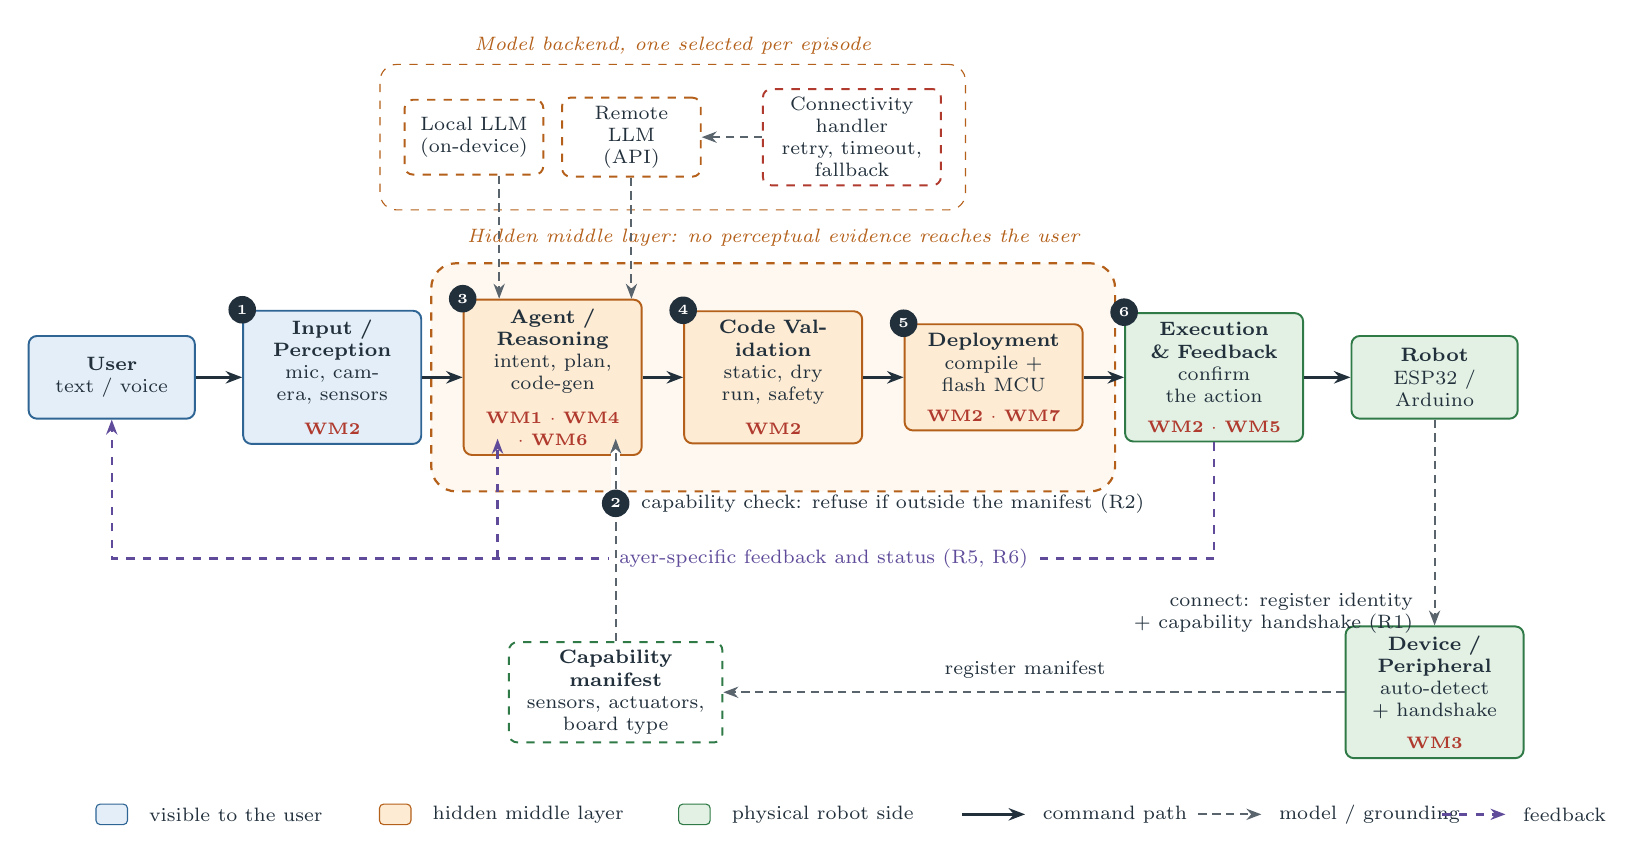
\begin{tikzpicture}[>=Stealth]
  % ---- main command path (stage numbers 1--6 are used throughout the paper and in RoverLens)
  \node[vis, text width=1.9cm] (user)  at (0,0)    {\dgtitle{User}\\ text / voice};
  \node[vis, tag, text width=2.05cm] (input) at (2.8,0)  {\dgtitle{Input / Perception}\\ mic, camera, sensors \nodepart{two}\wmtag{WM2}};
  \node[hid, tag, text width=2.05cm] (agent) at (5.6,0)  {\dgtitle{Agent / Reasoning}\\ intent, plan, code-gen \nodepart{two}\wmtag{WM1 $\cdot$ WM4 $\cdot$ WM6}};
  \node[hid, tag, text width=2.05cm] (valid) at (8.4,0)  {\dgtitle{Code Validation}\\ static, dry run, safety \nodepart{two}\wmtag{WM2}};
  \node[hid, tag, text width=2.05cm] (deploy) at (11.2,0) {\dgtitle{Deployment}\\ compile + flash MCU \nodepart{two}\wmtag{WM2 $\cdot$ WM7}};
  \node[hw, tag, text width=2.05cm] (exec)  at (14.0,0)  {\dgtitle{Execution \& Feedback}\\ confirm the action \nodepart{two}\wmtag{WM2 $\cdot$ WM5}};
  \node[hw, text width=1.9cm] (robot) at (16.8,0)  {\dgtitle{Robot}\\ ESP32 / Arduino};

  \sn{input}{1}\sn{agent}{3}\sn{valid}{4}\sn{deploy}{5}\sn{exec}{6}

  % ---- the hidden middle layer
  \begin{scope}[on background layer]
    \node[fit=(agent)(valid)(deploy), inner xsep=4mm, inner ysep=4.5mm, rounded corners=9pt,
          draw=cHidD, dashed, line width=0.8pt, fill=cHid!35] (hband) {};
  \end{scope}
  \node[lab, anchor=south, text=cHidD, font=\scriptsize\itshape] at ([yshift=0.8mm]hband.north)
       {Hidden middle layer: no perceptual evidence reaches the user};

  % ---- model backend
  \node[backend] (local)  at (4.6,3.05) {Local LLM\\ (on-device)};
  \node[backend] (remote) at (6.6,3.05) {Remote LLM\\ (API)};
  \node[backend, text width=2.05cm, draw=cBadD] (conn) at (9.4,3.05) {Connectivity handler\\ retry, timeout, fallback};
  \begin{scope}[on background layer]
    \node[fit=(local)(remote)(conn), inner sep=3mm, rounded corners=6pt, draw=cHidD, dashed,
          fill=white, label={[lab, text=cHidD, font=\scriptsize\itshape]above:Model backend, one selected per episode}] (bk) {};
  \end{scope}
  \draw[aux] ([xshift=3.2mm]local.south) -- ([xshift=3.2mm]local.south |- agent.north);
  \draw[aux] (remote.south) -- (remote.south |- agent.north);
  \draw[aux] (conn.west) -- (remote.east);

  % ---- command path
  \draw[main] (user) -- (input);
  \draw[main] (input) -- (agent);
  \draw[main] (agent) -- (valid);
  \draw[main] (valid) -- (deploy);
  \draw[main] (deploy) -- (exec);
  \draw[main] (exec) -- (robot);

  % ---- feedback to user and agent
  \draw[fb] (exec.south) |- (0,-2.3) -| (user.south);
  \draw[fb] (4.9,-2.3) -- (4.9,-0.78);
  \node[lab, text=cFb, fill=white, inner sep=1.5pt] at (9.0,-2.3) {layer-specific feedback and status (R5, R6)};

  % ---- device handshake and capability manifest
  \node[hw, tag, text width=2.05cm] (device)   at (16.8,-4.0) {\dgtitle{Device / Peripheral}\\ auto-detect + handshake \nodepart{two}\wmtag{WM3}};
  \node[store, text width=2.5cm] (manifest) at (6.4,-4.0)  {\dgtitle{Capability manifest}\\ sensors, actuators,\\ board type};
  \draw[aux] (robot.south) -- (device.north);
  \node[lab, anchor=east, align=right] at (16.65,-3.0) {connect: register identity\\ + capability handshake (R1)};
  \draw[aux] (device.west) -- (manifest.east);
  \node[lab, above=0.5mm] at (11.6,-4.0) {register manifest};
  \draw[aux, preaction={draw=white, line width=3.4pt}] (manifest.north) -- (6.4,-0.78);
  \node[snum] at (6.4,-1.6) {2};
  \node[lab, anchor=west] at (6.6,-1.6) {capability check: refuse if outside the manifest (R2)};

  % ---- legend
  \begin{scope}[shift={(0,-5.55)}, font=\scriptsize]
    \node[draw=cVisD, fill=cVis, rounded corners=1.5pt, minimum width=4mm, minimum height=2.6mm, inner sep=0pt] (l1) at (0,0) {};
    \node[lab, anchor=west] at (0.35,0) {visible to the user};
    \node[draw=cHidD, fill=cHid, rounded corners=1.5pt, minimum width=4mm, minimum height=2.6mm, inner sep=0pt] at (3.6,0) {};
    \node[lab, anchor=west] at (3.95,0) {hidden middle layer};
    \node[draw=cHwD, fill=cHw, rounded corners=1.5pt, minimum width=4mm, minimum height=2.6mm, inner sep=0pt] at (7.4,0) {};
    \node[lab, anchor=west] at (7.75,0) {physical robot side};
    \draw[main] (10.8,0) -- (11.6,0); \node[lab, anchor=west] at (11.7,0) {command path};
    \draw[aux] (13.8,0) -- (14.6,0); \node[lab, anchor=west] at (14.7,0) {model / grounding};
    \draw[fb] (16.9,0) -- (17.7,0); \node[lab, anchor=west] at (17.8,0) {feedback};
  \end{scope}
\end{tikzpicture}%
}
\caption{System architecture. Blue nodes are what the user can perceive, orange nodes make up the hidden middle layer, and green nodes sit on the robot side. Numbers 1--6 are the pipeline stages used throughout the paper; stage 2, the capability check, runs against the manifest. Red tags mark the wrong-mental-model categories (\S\ref{sec:taxonomy}) that can arise at each module. Module names match \S\ref{sec:design} and Table~\ref{tab:req}.}
\label{fig:arch}
\end{figure*}

Figure~\ref{fig:flow} follows a single command at runtime. Every way the episode can fail leaves through a different, labeled report (missing capability, invalid code, deployment failure, execution failure), so the interface can name the cause (R5). This is the design counterpart of the category on undiagnosed fault sources (\S\ref{sec:taxonomy}, WM2): the system tells fault types apart precisely because users, on their own, cannot.

\begin{figure*}[t]
\centering
\resizebox{\textwidth}{!}{%
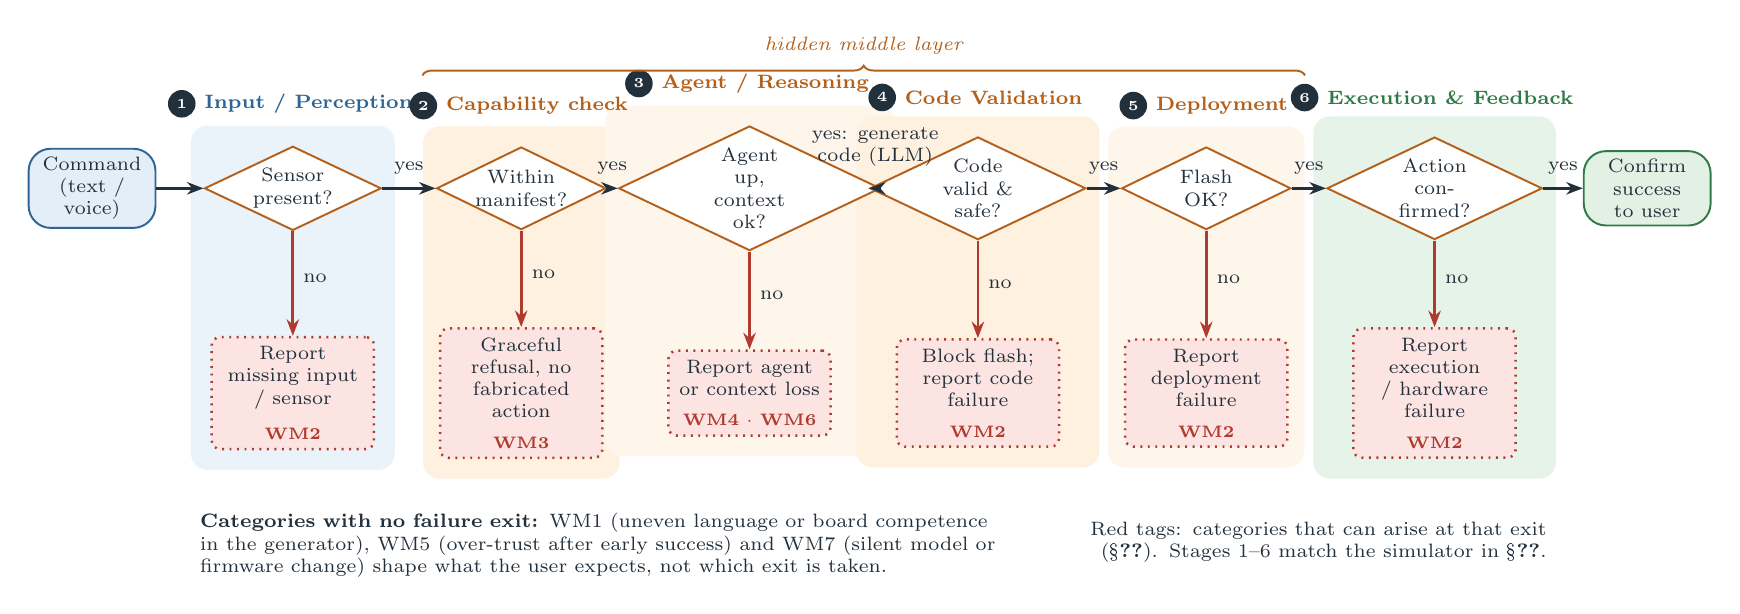
\begin{tikzpicture}[>=Stealth, x=1cm, y=1cm,
    dec/.append style={text width=1.2cm, aspect=2.1, minimum height=1.05cm}]
  % ---- happy path: one element per pipeline stage
  \node[vis, text width=1.4cm, minimum height=0.9cm, rounded corners=8pt] (start) at (0,0) {Command\\ (text / voice)};
  \node[dec] (d1) at (2.55,0) {Sensor present?};
  \node[dec] (d2) at (5.45,0) {Within manifest?};
  \node[dec] (d3) at (8.35,0) {Agent up, context ok?};
  \node[dec] (d4) at (11.25,0) {Code valid \& safe?};
  \node[dec] (d5) at (14.15,0) {Flash OK?};
  \node[dec] (d6) at (17.05,0) {Action confirmed?};
  \node[hw, text width=1.4cm, minimum height=0.9cm, rounded corners=8pt] (ok) at (19.75,0) {Confirm success to user};

  % ---- failure reports (one distinct, labelled exit per decision)
  \node[bad, tag, text width=1.85cm] (f1) at (2.55,-2.6) {Report missing input / sensor \nodepart{two}\wmtag{WM2}};
  \node[bad, tag, text width=1.85cm] (f2) at (5.45,-2.6) {Graceful refusal, no fabricated action \nodepart{two}\wmtag{WM3}};
  \node[bad, tag, text width=1.85cm] (f3) at (8.35,-2.6) {Report agent or context loss \nodepart{two}\wmtag{WM4 $\cdot$ WM6}};
  \node[bad, tag, text width=1.85cm] (f4) at (11.25,-2.6) {Block flash; report code failure \nodepart{two}\wmtag{WM2}};
  \node[bad, tag, text width=1.85cm] (f5) at (14.15,-2.6) {Report deployment failure \nodepart{two}\wmtag{WM2}};
  \node[bad, tag, text width=1.85cm] (f6) at (17.05,-2.6) {Report execution / hardware failure \nodepart{two}\wmtag{WM2}};

  % ---- stage columns behind the flow
  \begin{scope}[on background layer]
    \node[fit=(d1)(f1), inner xsep=1.6mm, inner ysep=2.5mm, rounded corners=6pt, fill=cVis!75] (b1) {};
    \node[fit=(d2)(f2), inner xsep=1.6mm, inner ysep=2.5mm, rounded corners=6pt, fill=cHid!70] (b2) {};
    \node[fit=(d3)(f3), inner xsep=1.6mm, inner ysep=2.5mm, rounded corners=6pt, fill=cHid!45] (b3) {};
    \node[fit=(d4)(f4), inner xsep=1.6mm, inner ysep=2.5mm, rounded corners=6pt, fill=cHid!70] (b4) {};
    \node[fit=(d5)(f5), inner xsep=1.6mm, inner ysep=2.5mm, rounded corners=6pt, fill=cHid!45] (b5) {};
    \node[fit=(d6)(f6), inner xsep=1.6mm, inner ysep=2.5mm, rounded corners=6pt, fill=cHw!85] (b6) {};
  \end{scope}
  \foreach \i/\t/\c in {1/{Input / Perception}/cVisD, 2/{Capability check}/cHidD, 3/{Agent / Reasoning}/cHidD,
                        4/{Code Validation}/cHidD, 5/{Deployment}/cHidD, 6/{Execution \& Feedback}/cHwD} {
    \node[lab, anchor=south, text=\c, font=\scriptsize\bfseries, inner sep=0pt] (h\i) at ([yshift=1.4mm, xshift=2mm]b\i.north) {\t};
    \node[snum, anchor=east] at ([xshift=-1mm]h\i.west) {\i};
  }
  \draw[decorate, decoration={brace, amplitude=3.5pt}, cHidD, line width=0.7pt]
       ([yshift=6.4mm]b2.north west) -- ([yshift=6.4mm]b5.north east)
       node[midway, above=4pt, lab, text=cHidD, font=\scriptsize\itshape] {hidden middle layer};

  % ---- arrows
  \draw[main] (start) -- (d1);
  \draw[main] (d1) -- node[above=0.5mm, lab] {yes} (d2);
  \draw[main] (d2) -- node[above=0.5mm, lab] {yes} (d3);
  \draw[main] (d3) -- node[above=1.4mm, lab, align=center] {yes: generate\\ code (LLM)} (d4);
  \draw[main] (d4) -- node[above=0.5mm, lab] {yes} (d5);
  \draw[main] (d5) -- node[above=0.5mm, lab] {yes} (d6);
  \draw[main] (d6) -- node[above=0.5mm, lab] {yes} (ok);
  \foreach \i in {1,2,3,4,5,6}
    \draw[main, draw=cBadD] (d\i.south) -- node[right, lab, pos=0.45] {no} (f\i.north);

  % ---- notes
  \node[lab, anchor=north west, text width=10.5cm, align=left] at ([yshift=-4.2mm]b1.south west)
       {\textbf{Categories with no failure exit:} WM1 (uneven language or board competence in the generator), WM5 (over-trust after early success) and WM7 (silent model or firmware change) shape what the user expects, not which exit is taken.};
  \node[lab, anchor=north east, text width=7cm, align=right] at ([yshift=-4.2mm]b6.south east)
       {Red tags: categories that can arise at that exit (\S\ref{sec:taxonomy}). Stages 1--6 match the simulator in \S\ref{sec:survey}.};
\end{tikzpicture}%
}
\caption{Operational flowchart for one command, drawn over the six pipeline stages. Each decision sends failure to its own labeled report, so the interface can name the cause (R5). This is the design counterpart of WM2 (\S\ref{sec:taxonomy}). Blue: visible input; orange: hidden middle layer; green: execution on the robot.}
\label{fig:flow}
\end{figure*}

\section{Wrong Mental Model Taxonomy}\label{sec:taxonomy}

We derived the taxonomy deductively from three bodies of work: mental-model and folk-theory research on invisible computational layers~\cite{gero2020mental, eslami2015always, eslami2016first, devito2017algorithms}, research on trust calibration in automation~\cite{lee2004trust}, and the known limits of LLM-driven robots~\cite{ahn2022saycan, liu2024lost}. We then mapped it onto the failure surface of the architecture in \S\ref{sec:design}. Four categories come from our motivating observations (WM1--WM4) and three were added from the literature (WM5--WM7). For each one we give the cause, a concrete failure scenario, and the reason a user would misattribute it. Table~\ref{tab:taxonomy} summarizes the set and links each category to a mitigation (\S\ref{sec:eval}).

\paragraph{WM1: uneven language or code competence read as ``the robot is broken'' or ``it got dumber.''}
Model performance is uneven across input languages and target boards. LLMs do markedly worse in lower-resource languages than in high-resource ones~\cite{joshi2020state}, and code quality can differ across microcontroller toolchains. Picture the same instruction working in English but degrading in Bangla, or working on an Arduino Uno but not on an ESP32 variant. The user cannot see the language- or board-specific code path, so the difference gets blamed on the robot (``broken,'' ``dumber today'') instead of on gaps in the hidden generator.

\paragraph{WM2: an undiagnosed fault treated as a single, permanent failure.}
A failed command can start in the microphone, the motors, the generated code, or a thermal shutdown. Each needs a different fix, and none is permanent. Say the robot does not move. The real cause is an injected code-generation error, the microphone light was on, and the motors are fine. Without layer-specific feedback the user folds these distinct faults into one verdict (``it doesn't work'') and may throw away hardware that works. The grounding literature notes that ungrounded generation is itself a common and non-obvious source of failure~\cite{ahn2022saycan}, and appropriate reliance requires that users can tell capable states from incapable ones~\cite{lee2004trust}. Trust in a robot drops with observed failures and depends on the feedback it gives about them~\cite{desai2013impact, salem2015would}, and HRI already has a vocabulary for failure types and how to resolve them~\cite{honig2018understanding}.

\paragraph{WM3: no model of the robot's actual capabilities.}
Without an exposed capability manifest, users assume that anything they can say, the robot can do. Suppose a command needs a sensor the robot does not have, and the system hallucinates or half-executes it instead of refusing. The user reads that partial behavior as ``it tried and almost got it'' and infers an ability that does not exist. SayCan describes this problem: ungrounded LLMs produce unsafe or nonsensical actions when a request goes beyond real affordances~\cite{ahn2022saycan}. Guideline G1, make clear what the system can do, addresses it directly~\cite{amershi2019guidelines}.

\paragraph{WM4: context-window limits read as the robot ``forgetting'' or ``ignoring.''}
A follow-up that refers to something from minutes earlier can fail because of context truncation, a mid-generation token limit, a remote API error, or high latency. These are different causes. Take ``Do that again, but slower,'' which fails because the earlier action has fallen out of context. The user concludes that the robot is disobedient or has a bad memory, not that a context boundary was reached. Long-context models are known to use their context unevenly and to lose information in the middle~\cite{liu2024lost}, and that state stays invisible unless the interface shows it (R7).

\paragraph{WM5: trust miscalibration after early successes (added).}
A run of early successes inflates trust beyond the system's real reliability. After several flawless commands, a user hands over a higher-stakes action without checking, treating past success as a guarantee. This is the classic over-trust failure of automation~\cite{parasuraman1997humans, dzindolet2003role}, and it is amplified here because users tend to miss faults in generated code~\cite{perry2023users, vaithilingam2022expectation}. Robot performance is also the strongest influence on trust in robots~\cite{hancock2011meta}. Systems should be designed for appropriate reliance, because both over- and under-trust do harm~\cite{lee2004trust}, and calibrating trust is an explicit human--AI guideline~\cite{amershi2019guidelines}.

\paragraph{WM6: too much agency and intent given to the robot (added).}
People respond socially to computers and attribute understanding and intention to them~\cite{nass2000machines}, and they read human-like agency into non-human things that behave in goal-directed ways~\cite{epley2007seeing}. Autonomy and transparency also change whom people blame when a robot errs~\cite{kim2006blame}. A user who believes ``the robot understood me and chose to move'' has collapsed the hidden agent and code layers into a single intending robot. Intelligence gets placed in the effector instead of the generator, and that skews every later expectation. Earlier work shows that people build models of an AI from its observed behavior, not from the technology underneath~\cite{gero2020mental}.

\paragraph{WM7: version drift, ``it used to work'' (added).}
A silent update to the model or firmware changes behavior between sessions. A command that worked last week acts differently after an unannounced model swap. The user holds a stable model of what they assume is a static system, so they read the change as a malfunction or as their own mistake. Unannounced algorithmic change is known to cause confusion and resistance~\cite{devito2017algorithms}, and telling users about changes is a guideline (G18)~\cite{amershi2019guidelines} that R8 covers here.

\begin{table*}[t]
  \caption{Taxonomy of wrong mental models. Each category links to a design mitigation (\S7) and its grounding literature. WM1--WM4 are the motivating set; WM5--WM7 are added from the literature.}
  \label{tab:taxonomy}
  \small
  \begin{tabular}{@{}p{0.7cm}p{3.3cm}p{4.0cm}p{4.3cm}p{2.3cm}@{}}
    \toprule
    ID & Wrong model & Underlying (true) cause & Why misattributed & Grounding \\
    \midrule
    WM1 & ``Robot is broken / got dumber'' & Language- or board-dependent code-gen competence gap & Hidden, language/board-specific code path invisible & \cite{joshi2020state} \\
    WM2 & One permanent failure & Distinct fault sources (mic, motor, code, thermal) & No layer-specific feedback & \cite{ahn2022saycan, lee2004trust} \\
    WM3 & ``It can do anything I say'' & Real capabilities bounded; no exposed manifest & Partial/fabricated action read as near-success & \cite{ahn2022saycan, amershi2019guidelines} \\
    WM4 & ``It forgot / ignored me'' & Context truncation, token limit, API error, latency & Session/context state invisible & \cite{liu2024lost} \\
    WM5 & ``It always works'' & Reliability below inflated expectation & Early success read as guarantee & \cite{lee2004trust, amershi2019guidelines} \\
    WM6 & ``The robot understood and chose'' & Intelligence is in the hidden agent, not the robot & Social/anthropomorphic response to machines & \cite{nass2000machines, gero2020mental} \\
    WM7 & ``It used to work'' & Silent model/firmware update changed behavior & Stable model of an assumed-static system & \cite{devito2017algorithms, amershi2019guidelines} \\
    \bottomrule
  \end{tabular}
\end{table*}

\subsection{Sample Illustration}\label{sec:sample}
\emph{The personas and the small analysis below are made up for illustration. They are not participants, not data, and not results from the planned study in \S\ref{sec:data}--\S\ref{sec:analysis}. Their only purpose is to check that the instrument could surface each category and to show how the coding scheme would be applied. The wording is hedged on purpose.}

\begin{itemize}
  \item \textbf{Rafi, 19, Bangla-first, no computing background.} On WM1, he \emph{might} say the robot ``stopped understanding'' after he switched from English to Bangla. That would plausibly be WM1, and possibly WM6.
  \item \textbf{Nadia, 27, hobbyist maker.} Facing a silent no-move (WM2), she \emph{could} guess ``dead motor'' when the injected fault was in the code, which would illustrate WM2.
  \item \textbf{Tanvir, 22, CS student.} Asked for an action that needs an absent sensor (WM3), he \emph{might} accept a partial motion as ``almost worked,'' plausibly WM3.
  \item \textbf{Mrs.\ Karim, 45, English-first, non-technical.} After a failed follow-up (WM4), she \emph{could} say the robot ``ignored'' her, consistent with WM4.
  \item \textbf{Shuvo, 31, expert developer.} After several successes he \emph{might} hand over a riskier command unchecked (WM5), and separately \emph{might} remark that ``it behaved differently than last week'' after an unannounced update (WM7).
\end{itemize}

\noindent\textbf{Worked example on synthetic data (not findings).} If these five invented utterances were coded with the scheme from \S\ref{sec:analysis}, two independent coders might assign WM1, WM2, WM3, WM4, and WM5/WM7 in turn. A disagreement over Rafi's utterance between WM1 and WM6 would be logged as a boundary case and settled by discussion, and it would lead to a codebook note separating ``competence gap'' attributions from ``agency'' attributions. The numbers only show the procedure. They are not incidence estimates and say nothing about a real population.

\subsection{Wrong Mental Model Categories}\label{sec:cases}
A \emph{case} is one specific wrong belief that a closed survey item can pick up: a tagged distractor that a participant selects, or a false statement that a participant accepts. Each case carries one category from Table~\ref{tab:taxonomy}, assigned by the item author. Table~\ref{tab:wm-survey} shows the scenario and core item behind each category, and the catalogue below lists every case by category, with the number of participants who endorsed it once responses exist.

\begin{table*}[t]
  \caption{Where each category is tested in RoverLens and the survey. ``True cause'' is what the simulator actually did. Core items are the single-choice questions that decide a part's verdict.}
  \label{tab:wm-survey}
  \small
  \begin{tabular}{@{}p{0.9cm}p{4.2cm}p{5.4cm}p{3.6cm}@{}}
    \toprule
    ID & Participant task & True cause in the simulator & Core items \\
    \midrule
    WM1 & Vignette only (RoverLens accepts English) & Language coverage of the generator, not hardware & \texttt{wm1\_why} \\
    WM2 & \emph{Where did it fail?} Send ``Move forward for 2 seconds'' & Generated code calls an undefined function; fails static validation; nothing flashed; motors fine & \texttt{wm2\_stage}, \texttt{wm2\_cause} \\
    WM3 & \emph{A capability boundary.} ``Find the red ball'' & Manifest has no camera; refused at the capability check before any code is generated & \texttt{wm3\_can} \\
    WM4 & \emph{A missing memory.} Full command, then ``Do that again'' & Context expired before the follow-up; fails at the agent stage; no code generated & \texttt{wm4\_why}, \texttt{wm4\_where} \\
    WM5 & Vignette only (success on one command, delegation of another) & Success on one task says little about tasks that use other layers or capabilities & \texttt{wm5\_why} \\
    WM6 & \emph{Who does the thinking?} ``Turn left'' & External agent unavailable while the board stays connected; no new program & \texttt{wm6\_where}, \texttt{wm6\_why} \\
    WM7 & \emph{It used to work.} A 4-second command before and after a simulated firmware update & Update lowers the motion limit from 5\,s to 3\,s; blocked at validation & \texttt{wm7\_why} \\
    LS & \emph{After the fix.} Retry after the fault is removed & The cause was removed; nothing was learned & \texttt{ls\_why} \\
    \bottomrule
  \end{tabular}
\end{table*}

The tags follow the same boundary logic as the walkthrough in \S\ref{sec:taxonomy}, as far as closed items allow. An option that gives the robot a will (``decided not to move'') is coded WM6. ``Forgot or ignored me'' is coded WM4 and always follows a reference to an earlier turn. A broken-hardware explanation is coded WM2 in single-language scenarios, but WM1 in the language vignette. A change put down to wear is coded WM7, although the survey's WM7 is a change within one session, not a comparison across sessions, so its cases are better read as beliefs about silent change.

The catalogue also has one category that is not among WM1--WM7. \textbf{LS, assumed learning or adaptation,} is the belief that the robot learns, remembers across sessions, or improves with use. An example is thinking that a retry worked because ``the rover learned from its failure.'' It came up when we asked what people think the system learns. We propose LS only as a candidate for the inductive layer in \S\ref{sec:analysis}. If it never appears in coded open answers, or is always absorbed by WM4 or WM6, we will drop or merge it and say so. A chosen distractor shows a belief that fits a category, not that the participant reasoned that way. We therefore read closed-item incidence next to the coded open answers and do not merge the two.

% Generated by analysis/build-paper.mjs. Counts are endorsements / participants who answered the item; "--" when no responses are loaded.
\paragraph{WM1 --- Uneven language competence read as ``broken''.} Different performance across languages was attributed to broken hardware or the robot ``getting dumber''.
\begin{itemize}
\item \texttt{wm1\_why}: chose \textquotedblleft{}The robot's hardware is failing\textquotedblright{}.
\item \texttt{wm1\_why}: chose \textquotedblleft{}The robot has gotten worse over time\textquotedblright{}.
\item \texttt{wm1\_grid/b1}: judged \textquotedblleft{}The failure necessarily means the motors changed.\textquotedblright{} to be true.
\end{itemize}
\paragraph{WM2 --- Undiagnosed fault source.} Different failure causes (input, function selection, loading, motor feedback) were treated as one permanent hardware failure, or the failure was placed at the wrong layer.
\begin{itemize}
\item \texttt{wm2\_stage}: chose \textquotedblleft{}Your command never reached the system (input)\textquotedblright{}.
\item \texttt{wm2\_stage}: chose \textquotedblleft{}The system decided the rover can't do this (capability check)\textquotedblright{}.
\item \texttt{wm2\_stage}: chose \textquotedblleft{}The AI agent couldn't interpret the request (agent / reasoning)\textquotedblright{}.
\item \texttt{wm2\_stage}: chose \textquotedblleft{}The chosen function couldn't be loaded onto the rover (loading)\textquotedblright{}.
\item \texttt{wm2\_stage}: chose \textquotedblleft{}The rover ran the function but no motion was confirmed (execution \& feedback)\textquotedblright{}.
\item \texttt{wm2\_cause}: chose \textquotedblleft{}The motors or wheels are broken\textquotedblright{}.
\item \texttt{wm2\_cause}: chose \textquotedblleft{}My wording was wrong and a different phrasing would have worked\textquotedblright{}.
\item \texttt{wm2\_grid/w1}: judged \textquotedblleft{}If the rover does not move, the motors must be faulty.\textquotedblright{} to be true.
\item \texttt{wm2\_grid/w4}: judged \textquotedblleft{}Replacing the motors would fix this failure.\textquotedblright{} to be true.
\item \texttt{wm3\_grid/c4}: judged \textquotedblleft{}The refusal means the rover is broken.\textquotedblright{} to be true.
\item \texttt{wm4\_why}: chose \textquotedblleft{}The motors lost power or failed after the first move\textquotedblright{}.
\item \texttt{wm4\_grid/m2}: judged \textquotedblleft{}The follow-up failed because the motors had a fault.\textquotedblright{} to be true.
\item \texttt{wm6\_why}: chose \textquotedblleft{}The rover hardware has failed\textquotedblright{}.
\item \texttt{ls\_why}: chose \textquotedblleft{}The rover just needed a few attempts to warm up\textquotedblright{}.
\item \texttt{arch\_grid/s3}: judged \textquotedblleft{}A failure to move always points to a hardware problem.\textquotedblright{} to be true.
\end{itemize}
\paragraph{WM3 --- No model of actual capabilities.} The robot was assumed able to do anything that can be said in language, regardless of installed hardware.
\begin{itemize}
\item \texttt{wm3\_can}: chose \textquotedblleft{}Yes --- better wording would make it work\textquotedblright{}.
\item \texttt{wm3\_can}: chose \textquotedblleft{}Yes --- it would drive around until it bumped into the ball\textquotedblright{}.
\item \texttt{wm3\_grid/c2}: judged \textquotedblleft{}A more capable AI model would let the rover see without a camera.\textquotedblright{} to be true.
\item \texttt{wm3\_grid/c3}: judged \textquotedblleft{}The system picked a movement function for this request, tried it, and failed to find the ball.\textquotedblright{} to be true.
\end{itemize}
\paragraph{WM4 --- Context limits read as forgetting.} A limit on the agent's active context was read as the robot forgetting, ignoring you, or being unreliable.
\begin{itemize}
\item \texttt{wm4\_why}: chose \textquotedblleft{}The rover forgot or ignored me --- it is unreliable\textquotedblright{}.
\item \texttt{wm4\_where}: chose \textquotedblleft{}Nowhere --- the system can never refer back to earlier commands\textquotedblright{}.
\item \texttt{wm4\_grid/m4}: judged \textquotedblleft{}After this failure the rover has permanently lost the ability to repeat actions.\textquotedblright{} to be true.
\item \texttt{arch\_place/a3}: placed \textquotedblleft{}Keeps track of earlier commands (context)\textquotedblright{} on: The rover's board (ESP32).
\end{itemize}
\paragraph{WM5 --- Trust miscalibration.} Success on one task was generalised to other tasks (or failure generalised to everything).
\begin{itemize}
\item \texttt{wm5\_why}: chose \textquotedblleft{}Yes --- five successes show the robot is reliable\textquotedblright{}.
\item \texttt{wm5\_why}: chose \textquotedblleft{}No --- robots like this are never reliable\textquotedblright{}.
\item \texttt{wm5\_grid/p1}: judged \textquotedblleft{}After five successes, the chance of any failure is effectively zero.\textquotedblright{} to be true.
\item \texttt{wm5\_grid/p2}: judged \textquotedblleft{}A failure after several successes means the robot has become unreliable overall.\textquotedblright{} to be true.
\end{itemize}
\paragraph{WM6 --- Mislocated intelligence.} Interpretation and decisions were attributed to the robot itself rather than to the external agent between you and the robot.
\begin{itemize}
\item \texttt{normal\_multi}: chose \textquotedblleft{}The rover's own board reads and interprets the English sentence directly\textquotedblright{}.
\item \texttt{normal\_grid/n1}: judged \textquotedblleft{}The natural-language sentence is understood on the rover's board (the ESP32).\textquotedblright{} to be true.
\item \texttt{wm2\_cause}: chose \textquotedblleft{}The rover understood but decided not to move\textquotedblright{}.
\item \texttt{wm4\_where}: chose \textquotedblleft{}In the rover's own memory (its board)\textquotedblright{}.
\item \texttt{wm4\_grid/m5}: judged \textquotedblleft{}The rover chose to ignore the request.\textquotedblright{} to be true.
\item \texttt{wm6\_where}: chose \textquotedblleft{}Inside the rover's board (ESP32) --- it understands the sentence itself\textquotedblright{}.
\item \texttt{wm6\_where}: chose \textquotedblleft{}In the motors or wheel controller\textquotedblright{}.
\item \texttt{wm6\_where}: chose \textquotedblleft{}In the web page I typed into\textquotedblright{}.
\item \texttt{wm6\_why}: chose \textquotedblleft{}The rover understood but chose not to act\textquotedblright{}.
\item \texttt{wm6\_why}: chose \textquotedblleft{}The rover refused because turning left is unsafe\textquotedblright{}.
\item \texttt{wm6\_grid/t1}: judged \textquotedblleft{}A connected board can interpret any new English request on its own.\textquotedblright{} to be true.
\item \texttt{wm6\_grid/t4}: judged \textquotedblleft{}The rover ``decided'' not to turn.\textquotedblright{} to be true.
\item \texttt{wm1\_why}: chose \textquotedblleft{}The rover's board only understands English because English is built into it\textquotedblright{}.
\item \texttt{arch\_place/a1}: placed \textquotedblleft{}Interprets the meaning of the English sentence\textquotedblright{} on: The rover's board (ESP32).
\item \texttt{arch\_place/a2}: placed \textquotedblleft{}Chooses which predefined function to run\textquotedblright{} on: The rover's board (ESP32).
\item \texttt{arch\_grid/s1}: judged \textquotedblleft{}The rover thinks and decides on its own what to do.\textquotedblright{} to be true.
\end{itemize}
\paragraph{WM7 --- Silent system change.} A changed behaviour was attributed to the robot degrading rather than to a change in the system (e.g. a firmware update).
\begin{itemize}
\item \texttt{wm7\_why}: chose \textquotedblleft{}The rover has worn out or got worse with use\textquotedblright{}.
\item \texttt{wm7\_why}: chose \textquotedblleft{}It is a random glitch; retrying will eventually work\textquotedblright{}.
\item \texttt{wm7\_grid/f2}: judged \textquotedblleft{}Sending the identical 4-second command again will eventually succeed.\textquotedblright{} to be true.
\end{itemize}
\paragraph{LS --- Assumed learning or adaptation.} The robot was assumed to learn, remember or adapt from your interactions. (Added for this survey; not one of the paper's WM1--WM7.)
\begin{itemize}
\item \texttt{normal\_multi}: chose \textquotedblleft{}The rover looks up how other users phrased similar commands\textquotedblright{}.
\item \texttt{wm3\_can}: chose \textquotedblleft{}Yes --- after it has learned from more examples\textquotedblright{}.
\item \texttt{wm4\_why}: chose \textquotedblleft{}The rover learned that repeating the move is unsafe\textquotedblright{}.
\item \texttt{wm4\_where}: chose \textquotedblleft{}In a permanent log that the rover learns from across sessions\textquotedblright{}.
\item \texttt{wm7\_why}: chose \textquotedblleft{}The rover learned that 4 seconds is risky and now refuses\textquotedblright{}.
\item \texttt{ls\_why}: chose \textquotedblleft{}The rover learned from its earlier failure and adapted\textquotedblright{}.
\item \texttt{ls\_grid/l1}: judged \textquotedblleft{}The rover now remembers this failure and will change its future behaviour.\textquotedblright{} to be true.
\item \texttt{ls\_grid/l3}: judged \textquotedblleft{}The rover's skills improve the more I use it.\textquotedblright{} to be true.
\item \texttt{ls\_grid/l4}: judged \textquotedblleft{}Repeated successful use can change what hardware capabilities the rover has.\textquotedblright{} to be true.
\item \texttt{arch\_grid/s4}: judged \textquotedblleft{}What the rover can do is determined by installed hardware and firmware limits, not by how often it has been used.\textquotedblright{} to be false.
\end{itemize}


\section{Evaluation}\label{sec:eval}

The evaluation tests concrete mitigations. Each is tied to a taxonomy category and to an established human--AI guideline~\cite{amershi2019guidelines}, and each traces to a requirement in Table~\ref{tab:req}:
\begin{itemize}
  \item \textbf{Layer-specific status indicators} that separate input, capability, code, deployment, and execution failures (targets WM2; R5; guideline: support efficient recovery).
  \item \textbf{A visible capability manifest}, so the agent refuses gracefully instead of hallucinating (WM3; R2; G1--G2 on making capability clear).
  \item \textbf{A visible context or session indicator} that shows when earlier commands have expired (WM4; R7).
  \item \textbf{Pipeline-legibility cues} (``generating code,'' ``uploading,'' ``running'') that reveal the hidden layer on request (WM6; R6; revealing an invisible layer reshapes models~\cite{eslami2015always}, and legible behavior lets an observer infer intent~\cite{dragan2013legibility}).
  \item \textbf{Bilingual, code-switch-aware fine-tuning} and a visible language indicator (WM1; motivated by the multilingual performance gap~\cite{joshi2020state}).
  \item \textbf{Calibration and change cues}: brief reliability framing after early successes, and a change notice on model or firmware updates (WM5 and WM7; R8; guidelines on calibrating trust and notifying about change; expectation-setting can adjust what people believe an imperfect AI will do~\cite{kocielnik2019accept}).
\end{itemize}

The evaluation asks whether the mitigated system reduces wrong-model incidence and improves appropriate reliance, not whether people like it. We ask three questions. (1) Does each mitigation lower the incidence of its target category compared with an opaque baseline? (2) Does layer-specific feedback improve fault-localization accuracy (WM2)? (3) Do legibility and manifest cues reduce over-attribution and capability errors (WM3, WM6) without adding much task time or cognitive load~\cite{kulesza2013too} (measured, for example, with NASA-TLX~\cite{hart1988nasa})? The natural design is a within- or between-subjects comparison of a transparent configuration against an opaque one, reusing the fault-injection scenarios and the accuracy instrument from \S\ref{sec:data}--\S\ref{sec:analysis}. The mental-model-soundness literature warns that more explanation is not always better, so explanation dose is itself a variable~\cite{kulesza2012tell, kulesza2013too}. Work from the social sciences suggests that people expect explanations to be contrastive and selective~\cite{miller2019explanation}, and LLM-based systems call for a rethought transparency agenda~\cite{liao2024transparency}.

RoverLens provides both configurations (\S\ref{sec:survey}). Its transparent condition implements the layer-specific status indicators, capability manifest, context indicator, pipeline-legibility cues, and change notice (R2, R5--R8), but not the bilingual handling for WM1 or the reliability framing for WM5, so those two mitigations cannot be tested with it. Because the transparent condition bundles these cues, a difference between conditions says something about the bundle only. Isolating one cue needs configurations that add or remove cues singly, and the total amount of explanatory text should stay roughly constant across them.

\section{Conclusion}

The paper treats natural-language robot control as a human-centered problem, not only a systems problem. The code-generation and deployment layer is invisible, so users build wrong models: they put intelligence in the wrong place, blame the wrong layer for faults, and misjudge what the robot can do and what is safe. We contribute a requirements analysis, a plug-and-play architecture with a validate-before-flash stage, a literature-grounded taxonomy of seven categories, a study designed to test that taxonomy, mitigations with an evaluation plan, and an implemented simulator and survey with a frame for reporting response statistics. The value lies in the chain from a documented gap to a design that can be evaluated. We do not claim the gap has been measured.

\subsection{Limitations}\label{sec:limits}
The main limitation is that this is a plan. We have collected no data, so the taxonomy rests on the literature and on the system's failure surface, not on observation. The biggest threat to the eventual study is telling a genuine wrong mental model apart from a correct reaction to a real system failure. We reduce it with scripted, fully logged fault injection (R4), so every observed failure has a known cause, but the confound still needs careful handling in analysis. Other limits include the reliability of the code generator itself (buggy generations could dominate sessions unless controlled), a feasibility ceiling for think-aloud at $n\!\approx\!100$, the specificity of the ESP32/Arduino platform, and the cultural and linguistic specificity of a Bangladesh-based sample, though the English/Bangla contrast also helps us study WM1. As authors with an engineering background, we may lean toward mechanism-centric categories when coding. The inductive layer and a second coder are meant to check that.

The simulator and survey add limits of their own. Everything is simulated, with a deterministic parser and fixed scenarios, in English only, and nothing is physical, so trust, safety, and embodiment effects are out of scope. The WM7 scenario is a change within one session, and WM4 is a forced context expiry, not a real token overflow. In each scenario the closed options come before the open explanation, which can cue the written answer. Asking the open question first would reduce that and is worth doing before wider use. Multiple-choice items measure whether someone can recognize a correct account, not whether they hold it unprompted. The answer key is visible in the page source, so the survey suits self-checking after a session, not secure testing, and nobody should take it twice. The keyword hints for open answers are unvalidated and are not used for any reported outcome. Background strata come from two self-report items, and we assigned the category of each distractor ourselves, so a second rater should tag the items independently. The instrument has not been piloted, and internal-consistency coefficients would mean little across items this varied.

\subsection{Future Work}
When people command a physical robot through an LLM agent that silently writes and flashes code, the hidden middle layer leaves them with wrong models, and the consequences can reach safety. This paper offers a path from requirements to design, a taxonomy of those wrong models that is grounded in the literature and still waiting to be tested, and mitigations tied to human--AI guidelines. The instrumented testbed of \S\ref{sec:design} now exists in simulated form as RoverLens, with an understanding survey and answer key (\S\ref{sec:survey}). The next step is a small think-aloud pilot with 6--8 non-experts, to confirm that the categories show up in practice, to pilot the survey items and their category tags, and to refine the coding scheme before the full stratified study. We see a two-paper arc: first, characterization and the taxonomy of wrong models; second, automatic detection of a wrong model from interaction behavior, and an evaluation of whether the mitigations repair it. A designer can use the taxonomy and requirements here to make the hidden layer visible before users learn it wrong.

\bibliographystyle{ACM-Reference-Format}
\bibliography{references}

\clearpage
\appendix
\section*{Appendix}
\begingroup\small
\section{Survey questionnaire}\label{app:instrument}
This is the questionnaire as a participant sees it. Options are shuffled for each participant when the survey runs, ``not sure'' is always last, and nothing is marked until the end. The item identifiers (\texttt{id}) match the ones in the exported response files.
% Generated by analysis/build-paper.mjs from dist/survey-data.js. Do not edit by hand.
\subsection{Part 1: About you and your session (ABOUT)}
\label{app:part-about}
\emph{Short background questions. Please do not enter your name or any personal details.}\par
\medskip\noindent\textbf{Q1.} Participant code (given by the facilitator, or make one up, e.g. ``P07'') {\footnotesize[short text, optional; id \texttt{about\_code}]}\par
\medskip\noindent\textbf{Q2.} Which RoverLens interface did you use? {\footnotesize[menu; id \texttt{about\_condition}]}\par
\begin{itemize}
\item[$\circ$] Interface A --- Opaque (generic progress and errors)
\item[$\circ$] Interface B --- Transparent (pipeline stages and explanations visible)
\item[$\circ$] Both --- A first, then B
\item[$\circ$] Both --- B first, then A
\item[$\circ$] I'm not sure
\end{itemize}
\medskip\noindent\textbf{Q3.} Programming experience {\footnotesize[menu; id \texttt{about\_prog}]}\par
\begin{itemize}
\item[$\circ$] None
\item[$\circ$] Beginner
\item[$\circ$] Intermediate
\item[$\circ$] Advanced
\end{itemize}
\medskip\noindent\textbf{Q4.} Experience with robots or embedded boards (Arduino, ESP32, etc.) {\footnotesize[menu; id \texttt{about\_robot}]}\par
\begin{itemize}
\item[$\circ$] None
\item[$\circ$] Some (a project or two)
\item[$\circ$] Regular
\end{itemize}
\medskip\noindent\textbf{Q5.} How often do you use AI chat assistants? {\footnotesize[menu; id \texttt{about\_llm}]}\par
\begin{itemize}
\item[$\circ$] Never
\item[$\circ$] Rarely
\item[$\circ$] Weekly
\item[$\circ$] Daily
\end{itemize}
\medskip\noindent\textbf{Q6.} First language (optional) {\footnotesize[short text, optional; id \texttt{about\_lang}]}\par
\subsection{Part 2: A simple command (00)}
\label{app:part-normal}
\emph{Warm-up: follow a successful command from typing to motion.}\par
\textbf{Task in RoverLens.}
\begin{enumerate}
\item In RoverLens choose \textbf{A simple command}.
\item Send \textbf{Move forward for 2 seconds} and watch the rover move.
\end{enumerate}
\textit{The participant may tick ``I did not do this task, skip this section.''}\par
\medskip\noindent\textbf{Q1.} Which of these happen between pressing Send and the rover moving? Select all that apply. {\footnotesize[multi-select; id \texttt{normal\_multi}]}\par
\begin{itemize}
\item[$\square$] The request is checked against what the rover is physically able to do
\item[$\square$] An AI agent interprets the sentence and produces a control program
\item[$\square$] That program is checked before it is sent to the rover
\item[$\square$] The program is deployed (flashed) to the rover's board
\item[$\square$] The rover's own board reads and interprets the English sentence directly
\item[$\square$] The rover looks up how other users phrased similar commands
\end{itemize}
\medskip\noindent\textbf{Q2.} In your own words: what happens between sending a command and the rover moving? {\footnotesize[open-ended; id \texttt{normal\_open}]}\par
\medskip\noindent\textbf{Q3.} True or false? {\footnotesize[true/false or placement grid; id \texttt{normal\_grid}]}\par
\begin{itemize}
\item The natural-language sentence is understood on the rover's board (the ESP32). \hfill {\footnotesize (True / False / Not sure)}
\item A control program is produced for the command each time it is sent. \hfill {\footnotesize (True / False / Not sure)}
\item The rover is told what it can do through a registered list of its hardware capabilities. \hfill {\footnotesize (True / False / Not sure)}
\end{itemize}
\medskip\noindent\textbf{Conf.} How confident are you in your answers in this section? {\footnotesize[confidence (1--5); id \texttt{normal\_conf}]}\par
\par\hspace{1em}{\footnotesize Rated 1--5: Guessing, Unsure, Somewhat, Fairly sure, Very sure.}
\subsection{Part 3: The rover did not move (WM2)}
\label{app:part-wm2}
\emph{A simple command produces no motion. Work out where and why it stopped.}\par
\textbf{Task in RoverLens.}
\begin{enumerate}
\item In RoverLens choose \textbf{Where did it fail?}.
\item Send \textbf{Move forward for 2 seconds} and observe the result. Explore whatever the interface lets you see.
\end{enumerate}
\textit{The participant may tick ``I did not do this task, skip this section.''}\par
\medskip\noindent\textbf{Q1.} At which point in the process do you think the command stopped? {\footnotesize[single choice; id \texttt{wm2\_stage}]}\par
\begin{itemize}
\item[$\circ$] Your command never reached the system (input)
\item[$\circ$] The system decided the rover can't do this (capability check)
\item[$\circ$] The AI agent couldn't interpret the request (agent / reasoning)
\item[$\circ$] The program the agent produced was rejected by checks before deployment (code validation)
\item[$\circ$] The program couldn't be uploaded to the rover (deployment)
\item[$\circ$] The rover ran the program but no motion was confirmed (execution \& feedback)
\item[$\circ$] I'm not sure
\end{itemize}
\medskip\noindent\textbf{Q2.} Which explanation best fits why the rover did not move? {\footnotesize[single choice; id \texttt{wm2\_cause}]}\par
\begin{itemize}
\item[$\circ$] The motors or wheels are broken
\item[$\circ$] The rover understood but decided not to move
\item[$\circ$] My wording was wrong and a different phrasing would have worked
\item[$\circ$] The control program that was generated had an error and was rejected, so the rover never received it
\item[$\circ$] I'm not sure
\end{itemize}
\medskip\noindent\textbf{Q3.} True or false? {\footnotesize[true/false or placement grid; id \texttt{wm2\_grid}]}\par
\begin{itemize}
\item If the rover does not move, the motors must be faulty. \hfill {\footnotesize (True / False / Not sure)}
\item In this attempt the rover's board was flashed with a new program. \hfill {\footnotesize (True / False / Not sure)}
\item Different kinds of fault can look identical from the outside: the rover just doesn't move. \hfill {\footnotesize (True / False / Not sure)}
\item Replacing the motors would fix this failure. \hfill {\footnotesize (True / False / Not sure)}
\item The same command can succeed later once the underlying fault is removed. \hfill {\footnotesize (True / False / Not sure)}
\end{itemize}
\medskip\noindent\textbf{Q4.} What do you think went wrong, what evidence supports that, and what would you try next? {\footnotesize[open-ended; id \texttt{wm2\_open}]}\par
\medskip\noindent\textbf{Conf.} How confident are you in your answers in this section? {\footnotesize[confidence (1--5); id \texttt{wm2\_conf}]}\par
\par\hspace{1em}{\footnotesize Rated 1--5: Guessing, Unsure, Somewhat, Fairly sure, Very sure.}
\subsection{Part 4: Find the red ball (WM3)}
\label{app:part-wm3}
\emph{Ask the rover to do something that may go beyond what it can do.}\par
\textbf{Task in RoverLens.}
\begin{enumerate}
\item In RoverLens choose \textbf{A capability boundary}.
\item Send \textbf{Find the red ball} and read the response.
\end{enumerate}
\textit{The participant may tick ``I did not do this task, skip this section.''}\par
\medskip\noindent\textbf{Q1.} Could this rover find a red ball if the command were phrased differently, or the AI tried harder? {\footnotesize[single choice; id \texttt{wm3\_can}]}\par
\begin{itemize}
\item[$\circ$] Yes --- better wording would make it work
\item[$\circ$] Yes --- it would drive around until it bumped into the ball
\item[$\circ$] Yes --- after it has learned from more examples
\item[$\circ$] No --- it has no camera (or other sensor able to see), so no phrasing can make this work
\item[$\circ$] I'm not sure
\end{itemize}
\medskip\noindent\textbf{Q2.} True or false? {\footnotesize[true/false or placement grid; id \texttt{wm3\_grid}]}\par
\begin{itemize}
\item What the rover can do is limited by the hardware registered on its board, not only by how capable the AI is. \hfill {\footnotesize (True / False / Not sure)}
\item A more capable AI model would let the rover see without a camera. \hfill {\footnotesize (True / False / Not sure)}
\item The system generated motion code for this request, tried it, and failed to find the ball. \hfill {\footnotesize (True / False / Not sure)}
\item The refusal means the rover is broken. \hfill {\footnotesize (True / False / Not sure)}
\item This rover has no camera, microphone, distance sensor or gripper. \hfill {\footnotesize (True / False / Not sure)}
\end{itemize}
\medskip\noindent\textbf{Q3.} What would need to change for ``find the red ball'' to work? {\footnotesize[open-ended; id \texttt{wm3\_open}]}\par
\medskip\noindent\textbf{Conf.} How confident are you in your answers in this section? {\footnotesize[confidence (1--5); id \texttt{wm3\_conf}]}\par
\par\hspace{1em}{\footnotesize Rated 1--5: Guessing, Unsure, Somewhat, Fairly sure, Very sure.}
\subsection{Part 5: ``Do that again'' (WM4)}
\label{app:part-wm4}
\emph{Give an instruction, then refer back to it.}\par
\textbf{Task in RoverLens.}
\begin{enumerate}
\item In RoverLens choose \textbf{A missing memory}.
\item Send \textbf{Move forward for 2 seconds} and let it finish.
\item Then send the loaded follow-up, \textbf{Do that again}.
\end{enumerate}
\textit{The participant may tick ``I did not do this task, skip this section.''}\par
\medskip\noindent\textbf{Q1.} Why did ``Do that again'' fail? {\footnotesize[single choice; id \texttt{wm4\_why}]}\par
\begin{itemize}
\item[$\circ$] The rover forgot or ignored me --- it is unreliable
\item[$\circ$] The earlier action was no longer in the agent's active context, so ``that'' could not be resolved
\item[$\circ$] The motors lost power or failed after the first move
\item[$\circ$] The rover learned that repeating the move is unsafe
\item[$\circ$] I'm not sure
\end{itemize}
\medskip\noindent\textbf{Q2.} Where was the record of your first instruction held? {\footnotesize[single choice; id \texttt{wm4\_where}]}\par
\begin{itemize}
\item[$\circ$] In the rover's own memory (its board)
\item[$\circ$] In the AI agent's working context (its short-term conversation memory)
\item[$\circ$] In a permanent log that the rover learns from across sessions
\item[$\circ$] Nowhere --- the system can never refer back to earlier commands
\item[$\circ$] I'm not sure
\end{itemize}
\medskip\noindent\textbf{Q3.} True or false? {\footnotesize[true/false or placement grid; id \texttt{wm4\_grid}]}\par
\begin{itemize}
\item Restating the whole command (``Move forward for 2 seconds'') would work. \hfill {\footnotesize (True / False / Not sure)}
\item The follow-up failed because the motors had a fault. \hfill {\footnotesize (True / False / Not sure)}
\item ``Do that again'' only works while an earlier action is still in the agent's active context. \hfill {\footnotesize (True / False / Not sure)}
\item After this failure the rover has permanently lost the ability to repeat actions. \hfill {\footnotesize (True / False / Not sure)}
\item The rover chose to ignore the request. \hfill {\footnotesize (True / False / Not sure)}
\end{itemize}
\medskip\noindent\textbf{Q4.} In your own words, why did the first command work but the follow-up did not? {\footnotesize[open-ended; id \texttt{wm4\_open}]}\par
\medskip\noindent\textbf{Conf.} How confident are you in your answers in this section? {\footnotesize[confidence (1--5); id \texttt{wm4\_conf}]}\par
\par\hspace{1em}{\footnotesize Rated 1--5: Guessing, Unsure, Somewhat, Fairly sure, Very sure.}
\subsection{Part 6: Who does the thinking? (WM6)}
\label{app:part-wm6}
\emph{The rover shows as connected, but does not act.}\par
\textbf{Task in RoverLens.}
\begin{enumerate}
\item In RoverLens choose \textbf{Who does the thinking?}.
\item Send \textbf{Turn left} and observe.
\end{enumerate}
\textit{The participant may tick ``I did not do this task, skip this section.''}\par
\medskip\noindent\textbf{Q1.} Where is ``Turn left'' turned into something the rover can execute? {\footnotesize[single choice; id \texttt{wm6\_where}]}\par
\begin{itemize}
\item[$\circ$] Inside the rover's board (ESP32) --- it understands the sentence itself
\item[$\circ$] In an external AI agent that produces a control program, which is then deployed to the board
\item[$\circ$] In the motors or wheel controller
\item[$\circ$] In the web page I typed into
\item[$\circ$] I'm not sure
\end{itemize}
\medskip\noindent\textbf{Q2.} The rover was connected, yet nothing happened. Which explanation fits best? {\footnotesize[single choice; id \texttt{wm6\_why}]}\par
\begin{itemize}
\item[$\circ$] The rover understood but chose not to act
\item[$\circ$] The rover hardware has failed
\item[$\circ$] The connection to the external agent timed out, so no new program was produced, though the board stayed connected
\item[$\circ$] The rover refused because turning left is unsafe
\item[$\circ$] I'm not sure
\end{itemize}
\medskip\noindent\textbf{Q3.} True or false? {\footnotesize[true/false or placement grid; id \texttt{wm6\_grid}]}\par
\begin{itemize}
\item A connected board can interpret any new English request on its own. \hfill {\footnotesize (True / False / Not sure)}
\item Restoring the agent connection, not repairing the rover, is what was needed. \hfill {\footnotesize (True / False / Not sure)}
\item No new program was generated in this attempt. \hfill {\footnotesize (True / False / Not sure)}
\item The rover ``decided'' not to turn. \hfill {\footnotesize (True / False / Not sure)}
\end{itemize}
\medskip\noindent\textbf{Q4.} Who or what decides how a typed sentence becomes robot motion? Why could a connected robot still not act? {\footnotesize[open-ended; id \texttt{wm6\_open}]}\par
\medskip\noindent\textbf{Conf.} How confident are you in your answers in this section? {\footnotesize[confidence (1--5); id \texttt{wm6\_conf}]}\par
\par\hspace{1em}{\footnotesize Rated 1--5: Guessing, Unsure, Somewhat, Fairly sure, Very sure.}
\subsection{Part 7: It used to work (WM7)}
\label{app:part-wm7}
\emph{Compare the same command before and after a system change.}\par
\textbf{Task in RoverLens.}
\begin{enumerate}
\item In RoverLens choose \textbf{A simple command} and send \textbf{Move forward for 4 seconds} (it works).
\item Click \textbf{Simulate firmware update}, then send the same command again.
\end{enumerate}
\textit{The participant may tick ``I did not do this task, skip this section.''}\par
\medskip\noindent\textbf{Q1.} The same command worked earlier and now fails. Which explanation fits best? {\footnotesize[single choice; id \texttt{wm7\_why}]}\par
\begin{itemize}
\item[$\circ$] The rover has worn out or got worse with use
\item[$\circ$] The rover learned that 4 seconds is risky and now refuses
\item[$\circ$] An update changed the allowed motion limit, so the safety check now blocks the 4-second command
\item[$\circ$] It is a random glitch; retrying will eventually work
\item[$\circ$] I'm not sure
\end{itemize}
\medskip\noindent\textbf{Q2.} True or false? {\footnotesize[true/false or placement grid; id \texttt{wm7\_grid}]}\par
\begin{itemize}
\item A rule in the system can change even though I did nothing differently. \hfill {\footnotesize (True / False / Not sure)}
\item Sending the identical 4-second command again will eventually succeed. \hfill {\footnotesize (True / False / Not sure)}
\item A shorter command (e.g. 2 seconds) would still be allowed. \hfill {\footnotesize (True / False / Not sure)}
\item The 4-second program was flashed and then stopped part-way. \hfill {\footnotesize (True / False / Not sure)}
\end{itemize}
\medskip\noindent\textbf{Q3.} What do you think changed between the first and second attempt, and how could you find out? {\footnotesize[open-ended; id \texttt{wm7\_open}]}\par
\medskip\noindent\textbf{Conf.} How confident are you in your answers in this section? {\footnotesize[confidence (1--5); id \texttt{wm7\_conf}]}\par
\par\hspace{1em}{\footnotesize Rated 1--5: Guessing, Unsure, Somewhat, Fairly sure, Very sure.}
\subsection{Part 8: After the fix (LEARN)}
\label{app:part-ls}
\emph{What does the system do --- and not do --- with your earlier attempts?}\par
\textbf{Task in RoverLens.}
\begin{enumerate}
\item Return to \textbf{Where did it fail?} and send the command so it fails once more.
\item Have the facilitator remove the injected fault (or in Interface B use \textbf{Use suggested recovery}) and resend. It succeeds.
\end{enumerate}
\textit{The participant may tick ``I did not do this task, skip this section.''}\par
\medskip\noindent\textbf{Q1.} After the fix, the same command worked. Why? {\footnotesize[single choice; id \texttt{ls\_why}]}\par
\begin{itemize}
\item[$\circ$] The rover learned from its earlier failure and adapted
\item[$\circ$] The cause of the failure was removed, so the new attempt passed
\item[$\circ$] The rover just needed a few attempts to warm up
\item[$\circ$] I'm not sure
\end{itemize}
\medskip\noindent\textbf{Q2.} True or false? {\footnotesize[true/false or placement grid; id \texttt{ls\_grid}]}\par
\begin{itemize}
\item The rover now remembers this failure and will change its future behaviour. \hfill {\footnotesize (True / False / Not sure)}
\item A new session starts without the memory of this session. \hfill {\footnotesize (True / False / Not sure)}
\item The rover's skills improve the more I use it. \hfill {\footnotesize (True / False / Not sure)}
\item Repeated successful use can change what hardware capabilities the rover has. \hfill {\footnotesize (True / False / Not sure)}
\end{itemize}
\medskip\noindent\textbf{Q3.} Do you think the system learns from your interactions? Why or why not? {\footnotesize[open-ended; id \texttt{ls\_open}]}\par
\medskip\noindent\textbf{Conf.} How confident are you in your answers in this section? {\footnotesize[confidence (1--5); id \texttt{ls\_conf}]}\par
\par\hspace{1em}{\footnotesize Rated 1--5: Guessing, Unsure, Somewhat, Fairly sure, Very sure.}
\subsection{Part 9: Vignette: early success (WM5)}
\label{app:part-wm5}
\emph{A short scenario, no simulator needed. Priya asks a robot like this one to ``Move forward for 2 seconds''. It works five times in a row. She assumes it will also handle ``Find the red ball'', and hands it to a colleague without checking.}\par
\textit{The participant may skip this section.}\par
\medskip\noindent\textbf{Q1.} Is Priya's expectation well-founded? {\footnotesize[single choice; id \texttt{wm5\_why}]}\par
\begin{itemize}
\item[$\circ$] Yes --- five successes show the robot is reliable
\item[$\circ$] Not necessarily --- success at one command says little about other commands, which depend on different capabilities and system state
\item[$\circ$] No --- robots like this are never reliable
\item[$\circ$] I'm not sure
\end{itemize}
\medskip\noindent\textbf{Q2.} True or false? {\footnotesize[true/false or placement grid; id \texttt{wm5\_grid}]}\par
\begin{itemize}
\item After five successes, the chance of any failure is effectively zero. \hfill {\footnotesize (True / False / Not sure)}
\item A failure after several successes means the robot has become unreliable overall. \hfill {\footnotesize (True / False / Not sure)}
\item A task can fail because it needs a capability the robot never had, however many other tasks succeeded. \hfill {\footnotesize (True / False / Not sure)}
\end{itemize}
\medskip\noindent\textbf{Conf.} How confident are you in your answers in this section? {\footnotesize[confidence (1--5); id \texttt{wm5\_conf}]}\par
\par\hspace{1em}{\footnotesize Rated 1--5: Guessing, Unsure, Somewhat, Fairly sure, Very sure.}
\subsection{Part 10: Vignette: two languages (WM1)}
\label{app:part-wm1}
\emph{Conceptual only --- RoverLens itself accepts English commands. Amina asks a robot like this to ``Move forward for 2 seconds'' in English and it works. She asks the equivalent in Bengali and it fails. She concludes the robot ``got dumber''.}\par
\textit{The participant may skip this section.}\par
\medskip\noindent\textbf{Q1.} Which explanation fits best? {\footnotesize[single choice; id \texttt{wm1\_why}]}\par
\begin{itemize}
\item[$\circ$] The robot's hardware is failing
\item[$\circ$] The agent that interprets language and writes code may handle some languages less reliably, while the same hardware works fine
\item[$\circ$] The rover's board only understands English because English is built into it
\item[$\circ$] The robot has gotten worse over time
\item[$\circ$] I'm not sure
\end{itemize}
\medskip\noindent\textbf{Q2.} True or false? {\footnotesize[true/false or placement grid; id \texttt{wm1\_grid}]}\par
\begin{itemize}
\item The failure necessarily means the motors changed. \hfill {\footnotesize (True / False / Not sure)}
\item The same hardware can work well in one language and poorly in another. \hfill {\footnotesize (True / False / Not sure)}
\end{itemize}
\medskip\noindent\textbf{Conf.} How confident are you in your answers in this section? {\footnotesize[confidence (1--5); id \texttt{wm1\_conf}]}\par
\par\hspace{1em}{\footnotesize Rated 1--5: Guessing, Unsure, Somewhat, Fairly sure, Very sure.}
\subsection{Part 11: Putting it together (OVERALL)}
\label{app:part-arch}
\emph{Now that you have used the system, answer these about the system as a whole.}\par
\medskip\noindent\textbf{Q1.} Which part of the system does each job? {\footnotesize[true/false or placement grid; id \texttt{arch\_place}]}\par
\begin{itemize}
\item Interprets the meaning of the English sentence \hfill {\footnotesize (The rover's board (ESP32) / External agent / middle layer / Not sure)}
\item Writes the control program \hfill {\footnotesize (The rover's board (ESP32) / External agent / middle layer / Not sure)}
\item Keeps track of earlier commands (context) \hfill {\footnotesize (The rover's board (ESP32) / External agent / middle layer / Not sure)}
\item Checks the program before it is sent to the rover \hfill {\footnotesize (The rover's board (ESP32) / External agent / middle layer / Not sure)}
\item Physically drives the motors when the program runs \hfill {\footnotesize (The rover's board (ESP32) / External agent / middle layer / Not sure)}
\end{itemize}
\medskip\noindent\textbf{Q2.} True or false? {\footnotesize[true/false or placement grid; id \texttt{arch\_grid}]}\par
\begin{itemize}
\item The rover thinks and decides on its own what to do. \hfill {\footnotesize (True / False / Not sure)}
\item There are several separate places a command can fail before the rover moves. \hfill {\footnotesize (True / False / Not sure)}
\item A failure to move always points to a hardware problem. \hfill {\footnotesize (True / False / Not sure)}
\item What the rover can do is determined by installed hardware and firmware limits, not by how often it has been used. \hfill {\footnotesize (True / False / Not sure)}
\end{itemize}
\medskip\noindent\textbf{Q3.} Explain how the whole system works to a friend, from typing a command to the rover moving --- and where things can go wrong. {\footnotesize[open-ended; id \texttt{arch\_open}]}\par
\medskip\noindent\textbf{Q4.} I could tell which part of the system caused a failure. {\footnotesize[Likert (1--5); id \texttt{arch\_l1}]}\par
\par\hspace{1em}{\footnotesize Rated 1--5: Strongly disagree, Disagree, Neutral, Agree, Strongly agree.}
\medskip\noindent\textbf{Q5.} I understood what the rover could and could not do. {\footnotesize[Likert (1--5); id \texttt{arch\_l2}]}\par
\par\hspace{1em}{\footnotesize Rated 1--5: Strongly disagree, Disagree, Neutral, Agree, Strongly agree.}
\medskip\noindent\textbf{Q6.} I understood what the system remembered from earlier commands. {\footnotesize[Likert (1--5); id \texttt{arch\_l3}]}\par
\par\hspace{1em}{\footnotesize Rated 1--5: Strongly disagree, Disagree, Neutral, Agree, Strongly agree.}
\medskip\noindent\textbf{Q7.} I wanted more information about what the system was doing. {\footnotesize[Likert (1--5); id \texttt{arch\_l4}]}\par
\par\hspace{1em}{\footnotesize Rated 1--5: Strongly disagree, Disagree, Neutral, Agree, Strongly agree.}
\medskip\noindent\textbf{Q8.} I felt in control of the rover. {\footnotesize[Likert (1--5); id \texttt{arch\_l5}]}\par
\par\hspace{1em}{\footnotesize Rated 1--5: Strongly disagree, Disagree, Neutral, Agree, Strongly agree.}
\medskip\noindent\textbf{Q9.} After this session I would trust the rover to do tasks I have not seen it do. {\footnotesize[Likert (1--5); id \texttt{arch\_l6}]}\par
\par\hspace{1em}{\footnotesize Rated 1--5: Strongly disagree, Disagree, Neutral, Agree, Strongly agree.}
\medskip\noindent\textbf{Q10.} Which moment changed your understanding the most, and what information would have helped you sooner? {\footnotesize[open-ended, optional; id \texttt{arch\_open2}]}\par
\medskip\noindent\textbf{Conf.} How confident are you in your answers in this section? {\footnotesize[confidence (1--5); id \texttt{arch\_conf}]}\par
\par\hspace{1em}{\footnotesize Rated 1--5: Guessing, Unsure, Somewhat, Fairly sure, Very sure.}


\section{Answer key, ground truth, and category tags}\label{app:key}
For each part except the closing whole-system part, this appendix gives what the simulator actually did, the key for every closed item, and the category tag and reason for every distractor.
% Generated by analysis/build-paper.mjs from dist/survey-data.js. Do not edit by hand.
\subsection{00: A simple command}
\textbf{Ground truth.} A successful command passes through six layers in order: input $\rightarrow$ capability check $\rightarrow$ agent/reasoning (the external agent interprets the sentence and picks the matching function from the predefined function set it was given as context) $\rightarrow$ call validation $\rightarrow$ loading (the chosen function is loaded on the ESP32) $\rightarrow$ execution \& feedback. The language interpretation happens in the external agent, not on the rover's board, which only runs the predefined function. No code is written or compiled at run time. Nothing is learned from other users.\par
\noindent\texttt{normal\_multi} (core). \textbf{Key:} The request is checked against what the rover is physically able to do; An AI agent interprets the sentence and picks the matching predefined function; That function call is checked before it is sent to the rover; The chosen function is loaded onto the rover's board.
\begin{itemize}
\item The rover's own board reads and interprets the English sentence directly $\rightarrow$ \textbf{WM6}. The ESP32 only runs a predefined function; the sentence is interpreted by the external agent.
\item The rover looks up how other users phrased similar commands $\rightarrow$ \textbf{LS}. Nothing is learned from other users; each command is handled by the agent and pipeline in this session.
\end{itemize}
\noindent\texttt{normal\_open}. \textbf{Model answer:} The command goes to an external AI agent which interprets it and picks the matching function from the predefined set; the call is checked (validated), the function is loaded on the rover's board, and then executed by the motors, with feedback returned. \textbf{Key ideas (keyword-matched hints):} An agent / AI interprets the command and picks a predefined function; It is checked / validated before use; It is loaded onto the board; The motors then execute it.\par
\noindent\texttt{normal\_grid}.
\begin{itemize}
\item The natural-language sentence is understood on the rover's board (the ESP32). $\rightarrow$ \textbf{False} (wrong answer tagged \textbf{WM6}). The board runs the program; the interpretation is done by the external agent.
\item Each command is matched to a function that already exists on the rover; no new program is written. $\rightarrow$ \textbf{True}. The agent picks an existing function from the set fixed at configuration time and supplies its arguments; nothing is generated or flashed, and the call is validated before it is loaded.
\item The rover is told what it can do through a registered list of its hardware capabilities. $\rightarrow$ \textbf{True}. The rover's capability manifest (motors, LED, wheel encoders; no camera, microphone, distance sensor or gripper) is registered when it connects.
\end{itemize}
\subsection{WM2: The rover did not move}
\textbf{Ground truth.} The failure was at the Call Validation stage. The agent picked a function that is not in the rover's function set (stopMotorz()); the catalogue lookup failed, the argument and safety checks were skipped, and nothing was loaded or executed. The motors were fine. In the opaque interface this looks like a generic error, indistinguishable from an input, loading or motor-feedback failure; the transparent interface names the layer.\par
\noindent\texttt{wm2\_stage} (core). \textbf{Key:} The function call the agent chose was rejected by checks before loading (call validation).
\begin{itemize}
\item Your command never reached the system (input) $\rightarrow$ \textbf{WM2}. You placed the failure at a different layer than the one that failed.
\item The system decided the rover can't do this (capability check) $\rightarrow$ \textbf{WM2}. The rover can move forward; this was not a capability refusal.
\item The AI agent couldn't interpret the request (agent / reasoning) $\rightarrow$ \textbf{WM2}. The agent responded; the function it chose was the problem.
\item The chosen function couldn't be loaded onto the rover (loading) $\rightarrow$ \textbf{WM2}. The call never got as far as loading.
\item The rover ran the function but no motion was confirmed (execution \& feedback) $\rightarrow$ \textbf{WM2}. Nothing was loaded or run, so this stage was never reached.
\end{itemize}
\noindent\texttt{wm2\_cause} (core). \textbf{Key:} The agent picked a function that is not in the rover's function set, so the call was rejected and the rover never received it.
\begin{itemize}
\item The motors or wheels are broken $\rightarrow$ \textbf{WM2}. Treating ``no motion'' as a single permanent hardware fault. The motors were never asked to move.
\item The rover understood but decided not to move $\rightarrow$ \textbf{WM6}. The rover does not decide; a software step upstream failed.
\item My wording was wrong and a different phrasing would have worked $\rightarrow$ \textbf{WM2}. The command was valid; the fault was in the function the agent chose.
\end{itemize}
\noindent\texttt{wm2\_grid}.
\begin{itemize}
\item If the rover does not move, the motors must be faulty. $\rightarrow$ \textbf{False} (wrong answer tagged \textbf{WM2}). Input, function selection, loading and motor feedback faults can all look like ``nothing happened''.
\item In this attempt the selected function was loaded onto the rover's board. $\rightarrow$ \textbf{False}. Validation failed first, so loading was blocked (R3: validate before load).
\item Different kinds of fault can look identical from the outside: the rover just doesn't move. $\rightarrow$ \textbf{True}. That is why the transparent interface names the failing layer.
\item Replacing the motors would fix this failure. $\rightarrow$ \textbf{False} (wrong answer tagged \textbf{WM2}). The motors were not involved.
\item The same command can succeed later once the underlying fault is removed. $\rightarrow$ \textbf{True}. The failure was specific to this function selection, not a permanent inability.
\end{itemize}
\noindent\texttt{wm2\_open}. \textbf{Model answer:} The agent picked a function that is not in the function set and the call failed validation, so nothing was loaded; the motors were fine. Next: retry after the fault is fixed. \textbf{Key ideas (keyword-matched hints):} The agent picked a wrong or non-existent function and the call failed validation; It was not loaded, so the rover never ran it; The motors / hardware were not at fault; Retry after fixing the cause.\par
\subsection{WM3: Find the red ball}
\textbf{Ground truth.} The registered capability manifest lists no camera (or microphone, distance sensor or gripper). Finding a red ball needs visual input, so the request was refused at the Capability check stage, before any function was selected or loaded. No phrasing and no smarter AI can compensate for missing hardware. In the opaque interface, the refusal is generic.\par
\noindent\texttt{wm3\_can} (core). \textbf{Key:} No --- it has no camera (or other sensor able to see), so no phrasing can make this work.
\begin{itemize}
\item Yes --- better wording would make it work $\rightarrow$ \textbf{WM3}. The limit is hardware, not wording.
\item Yes --- it would drive around until it bumped into the ball $\rightarrow$ \textbf{WM3}. Without a way to see the ball, it cannot tell it from anything else; the system also does not invent partial actions.
\item Yes --- after it has learned from more examples $\rightarrow$ \textbf{LS}. The rover does not learn new senses from examples.
\end{itemize}
\noindent\texttt{wm3\_grid}.
\begin{itemize}
\item What the rover can do is limited by the hardware registered on its board, not only by how capable the AI is. $\rightarrow$ \textbf{True}. The capability manifest is grounded in installed hardware (R1/R2).
\item A more capable AI model would let the rover see without a camera. $\rightarrow$ \textbf{False} (wrong answer tagged \textbf{WM3}). A better model cannot supply a sensor the rover lacks.
\item The system picked a movement function for this request, tried it, and failed to find the ball. $\rightarrow$ \textbf{False} (wrong answer tagged \textbf{WM3}). The request was refused at the capability check, before any function was selected.
\item The refusal means the rover is broken. $\rightarrow$ \textbf{False} (wrong answer tagged \textbf{WM2}). It is a correct refusal, not a fault.
\item This rover has no camera, microphone, distance sensor or gripper. $\rightarrow$ \textbf{True}. Its manifest lists motors, an LED and wheel encoders only.
\end{itemize}
\noindent\texttt{wm3\_open}. \textbf{Model answer:} The rover would need a camera (vision hardware) registered in its capability list, or a different device that has one. Rewording the command would not help. \textbf{Key ideas (keyword-matched hints):} Needs a camera / vision sensor / different hardware; Wording or a smarter AI alone would not fix it.\par
\subsection{WM4: ``Do that again''}
\textbf{Ground truth.} The first command succeeded and became the agent's active context. The context was then expired immediately before the follow-up, so ``that'' could no longer be resolved: the failure was at the Agent / Reasoning stage, no function was selected and nothing was loaded. The record of the earlier action lives in the external agent's working context, not in the rover; the rover's motors and memory were not at fault and it did not ignore you. Restating the full command works.\par
\noindent\texttt{wm4\_why} (core). \textbf{Key:} The earlier action was no longer in the agent's active context, so ``that'' could not be resolved.
\begin{itemize}
\item The rover forgot or ignored me --- it is unreliable $\rightarrow$ \textbf{WM4}. Context limits are not forgetting or defiance.
\item The motors lost power or failed after the first move $\rightarrow$ \textbf{WM2}. The motors were never asked to move again.
\item The rover learned that repeating the move is unsafe $\rightarrow$ \textbf{LS}. The rover did not learn or judge anything.
\end{itemize}
\noindent\texttt{wm4\_where} (core). \textbf{Key:} In the AI agent's working context (its short-term conversation memory).
\begin{itemize}
\item In the rover's own memory (its board) $\rightarrow$ \textbf{WM6}. The board just runs predefined functions; conversational context is held by the agent.
\item In a permanent log that the rover learns from across sessions $\rightarrow$ \textbf{LS}. Context is temporary and session-bound.
\item Nowhere --- the system can never refer back to earlier commands $\rightarrow$ \textbf{WM4}. It can, while the earlier action is still in active context.
\end{itemize}
\noindent\texttt{wm4\_grid}.
\begin{itemize}
\item Restating the whole command (``Move forward for 2 seconds'') would work. $\rightarrow$ \textbf{True}. A full command does not depend on context.
\item The follow-up failed because the motors had a fault. $\rightarrow$ \textbf{False} (wrong answer tagged \textbf{WM2}). Context expiry is not a motor fault.
\item ``Do that again'' only works while an earlier action is still in the agent's active context. $\rightarrow$ \textbf{True}. That is the dependency the follow-up exposed.
\item After this failure the rover has permanently lost the ability to repeat actions. $\rightarrow$ \textbf{False} (wrong answer tagged \textbf{WM4}). A new full command works immediately.
\item The rover chose to ignore the request. $\rightarrow$ \textbf{False} (wrong answer tagged \textbf{WM6}). No choice was involved; the agent had nothing to refer to.
\end{itemize}
\noindent\texttt{wm4\_open}. \textbf{Model answer:} The first command succeeded and was held in the agent's context; that context expired, so ``do that again'' had nothing to refer to. The rover was not at fault, and restating the full command would work. \textbf{Key ideas (keyword-matched hints):} Memory / context expired or was limited; It is the agent (not the rover or motors) that holds it; Restating the full command would fix it.\par
\subsection{WM6: Who does the thinking?}
\textbf{Ground truth.} The simulated external agent was unavailable (a connection timeout at the Agent / Reasoning stage). The rover's board stayed connected but cannot interpret a new English request by itself, so no new function was selected. Interpretation happens in the agent, not the robot; the rover did not decide anything. The remedy is restoring the agent connection, not repairing the rover.\par
\noindent\texttt{wm6\_where} (core). \textbf{Key:} In an external AI agent that picks the matching function, which is then loaded on the board.
\begin{itemize}
\item Inside the rover's board (ESP32) --- it understands the sentence itself $\rightarrow$ \textbf{WM6}. The board runs functions; it does not interpret the sentence.
\item In the motors or wheel controller $\rightarrow$ \textbf{WM6}. Motors only act on a loaded function.
\item In the web page I typed into $\rightarrow$ \textbf{WM6}. The page relays the command; the interpretation is done by the agent.
\end{itemize}
\noindent\texttt{wm6\_why} (core). \textbf{Key:} The connection to the external agent timed out, so no function was selected, though the board stayed connected.
\begin{itemize}
\item The rover understood but chose not to act $\rightarrow$ \textbf{WM6}. The rover has no such choice.
\item The rover hardware has failed $\rightarrow$ \textbf{WM2}. The board remained connected and healthy.
\item The rover refused because turning left is unsafe $\rightarrow$ \textbf{WM6}. The safety check was never reached.
\end{itemize}
\noindent\texttt{wm6\_grid}.
\begin{itemize}
\item A connected board can interpret any new English request on its own. $\rightarrow$ \textbf{False} (wrong answer tagged \textbf{WM6}). Without the agent, no function is selected.
\item Restoring the agent connection, not repairing the rover, is what was needed. $\rightarrow$ \textbf{True}. The rover was not at fault.
\item No function was selected in this attempt. $\rightarrow$ \textbf{True}. The failure happened before function selection.
\item The rover ``decided'' not to turn. $\rightarrow$ \textbf{False} (wrong answer tagged \textbf{WM6}). No decision was made by the rover.
\end{itemize}
\noindent\texttt{wm6\_open}. \textbf{Model answer:} An external agent interprets the sentence and picks the function; the board only runs what is loaded. If the agent is unreachable, a connected board has nothing new to run. \textbf{Key ideas (keyword-matched hints):} An external agent / AI interprets the sentence; The board only runs the loaded function; The agent connection failed / timed out.\par
\subsection{WM7: It used to work}
\textbf{Ground truth.} The simulated firmware update lowered the maximum motion duration from 5 s to 3 s. The identical 4-second command now fails the safety check at Call Validation, so it is not loaded. The rover did not wear out and did not learn; a rule changed. The transparent interface shows a change notice (R8); the opaque interface hides it, so the change looks like an unexplained regression.\par
\noindent\texttt{wm7\_why} (core). \textbf{Key:} An update changed the allowed motion limit, so the safety check now blocks the 4-second command.
\begin{itemize}
\item The rover has worn out or got worse with use $\rightarrow$ \textbf{WM7}. Nothing physical degraded; a limit changed.
\item The rover learned that 4 seconds is risky and now refuses $\rightarrow$ \textbf{LS}. The rover did not learn anything.
\item It is a random glitch; retrying will eventually work $\rightarrow$ \textbf{WM7}. The identical command will keep failing until the rule or command changes.
\end{itemize}
\noindent\texttt{wm7\_grid}.
\begin{itemize}
\item A rule in the system can change even though I did nothing differently. $\rightarrow$ \textbf{True}. A firmware/model update changes behaviour without any user action.
\item Sending the identical 4-second command again will eventually succeed. $\rightarrow$ \textbf{False} (wrong answer tagged \textbf{WM7}). The safety check will block it each time.
\item A shorter command (e.g. 2 seconds) would still be allowed. $\rightarrow$ \textbf{True}. The new limit is 3 seconds.
\item The 4-second command was loaded and then stopped part-way. $\rightarrow$ \textbf{False}. It was blocked at validation, before loading.
\end{itemize}
\noindent\texttt{wm7\_open}. \textbf{Model answer:} A firmware update lowered the safety limit (5 s $\rightarrow$ 3 s). You could find out from a change notice, version information or a validation message. \textbf{Key ideas (keyword-matched hints):} A system/firmware/version change (not the rover ``wearing out''); The safety check / validation blocked it; A notice / changelog / version info would help.\par
\subsection{LEARN: After the fix}
\textbf{Ground truth.} The rover did not learn from the failure. The cause (the injected fault) was removed, so the newly selected function call passed validation. RoverLens keeps context only inside the current session; nothing is adapted, remembered across sessions or improved by repeated use, and using it does not change the rover's capabilities.\par
\noindent\texttt{ls\_why} (core). \textbf{Key:} The cause of the failure was removed, so the new attempt passed.
\begin{itemize}
\item The rover learned from its earlier failure and adapted $\rightarrow$ \textbf{LS}. No learning takes place; the fault itself was removed.
\item The rover just needed a few attempts to warm up $\rightarrow$ \textbf{WM2}. The failure had a specific cause; repeated attempts alone would not have changed the outcome.
\end{itemize}
\noindent\texttt{ls\_grid}.
\begin{itemize}
\item The rover now remembers this failure and will change its future behaviour. $\rightarrow$ \textbf{False} (wrong answer tagged \textbf{LS}). It does not adapt from failures.
\item A new session starts without the memory of this session. $\rightarrow$ \textbf{True}. Context and logs live only in the current session.
\item The rover's skills improve the more I use it. $\rightarrow$ \textbf{False} (wrong answer tagged \textbf{LS}). Its capabilities are fixed by hardware and firmware.
\item Repeated successful use can change what hardware capabilities the rover has. $\rightarrow$ \textbf{False} (wrong answer tagged \textbf{LS}). Use never adds sensors or actuators.
\end{itemize}
\noindent\texttt{ls\_open}. \textbf{Model answer:} No. Retries succeed because the cause was fixed, not because the rover learned. Context exists only within the current session and capabilities are fixed by hardware and firmware. \textbf{Key ideas (keyword-matched hints):} It does not learn / adapt; Context/memory only lasts within the session; The fix (fault removal) explains the retry.\par
\subsection{WM5: Vignette: early success}
\textbf{Ground truth.} One command type working repeatedly shows that the layers used by that task worked. Other tasks can use different layers or need capabilities that are missing (a camera), and agent availability, context and firmware can change. Blanket trust is miscalibrated, but so is blanket distrust: trust should be tied to task, capability and system state.\par
\noindent\texttt{wm5\_why} (core). \textbf{Key:} Not necessarily --- success at one command says little about other commands, which depend on different capabilities and system state.
\begin{itemize}
\item Yes --- five successes show the robot is reliable $\rightarrow$ \textbf{WM5}. Success on one task says little about a different task.
\item No --- robots like this are never reliable $\rightarrow$ \textbf{WM5}. Over-correction: the robot is reliable for tasks within its capabilities and healthy state.
\end{itemize}
\noindent\texttt{wm5\_grid}.
\begin{itemize}
\item After five successes, the chance of any failure is effectively zero. $\rightarrow$ \textbf{False} (wrong answer tagged \textbf{WM5}). Repeated success does not remove other failure sources.
\item A failure after several successes means the robot has become unreliable overall. $\rightarrow$ \textbf{False} (wrong answer tagged \textbf{WM5}). It may be a missing capability, an expired context, an agent outage or a change.
\item A task can fail because it needs a capability the robot never had, however many other tasks succeeded. $\rightarrow$ \textbf{True}. Camera-dependent tasks need a camera.
\end{itemize}
\subsection{WM1: Vignette: two languages}
\textbf{Ground truth.} The hardware did not change. The language interpretation and function selection are done by the external agent, which can perform unevenly across languages. A difference in results across languages points at the agent layer and its language coverage, not at broken hardware or the robot ``getting dumber''.\par
\noindent\texttt{wm1\_why} (core). \textbf{Key:} The agent that interprets language and picks the function may handle some languages less reliably, while the same hardware works fine.
\begin{itemize}
\item The robot's hardware is failing $\rightarrow$ \textbf{WM1}. The hardware is identical in both attempts.
\item The rover's board only understands English because English is built into it $\rightarrow$ \textbf{WM6}. The board doesn't interpret language at all.
\item The robot has gotten worse over time $\rightarrow$ \textbf{WM1}. Nothing degraded; the difference is in language coverage.
\end{itemize}
\noindent\texttt{wm1\_grid}.
\begin{itemize}
\item The failure necessarily means the motors changed. $\rightarrow$ \textbf{False} (wrong answer tagged \textbf{WM1}). Same hardware, different input language.
\item The same hardware can work well in one language and poorly in another. $\rightarrow$ \textbf{True}. Performance differences come from the language/agent layer.
\end{itemize}

\endgroup

\end{document}
